\documentclass[12pt]{article}

% =========================================================================
% Preamble compartilhado - Nota PNADC (working paper format)
% =========================================================================
% Author: Vitor Pereira
% Last update: 2026-06-24
%
% Carrega pacotes basicos para working paper economico padrao:
%   - 12pt article, margins 1in, doublespacing body, singlespacing abstract/refs
%   - titling para tamanho correto de titulo (\large, nao default \Large)
%   - amsmath, natbib (authoryear,round), booktabs, threeparttable, hyperref
% =========================================================================

\usepackage[utf8]{inputenc}
\usepackage[T1]{fontenc}
\usepackage[brazilian]{babel}

\usepackage{geometry}
\geometry{margin=1in}

\usepackage{setspace}

\usepackage{amsmath, amssymb, amsthm}
\usepackage{graphicx}
\usepackage{booktabs}
\usepackage{threeparttable}
\usepackage{multirow}
\usepackage{array}
\usepackage{tabularx}
\usepackage{caption}
\usepackage{subcaption}
\usepackage{tcolorbox}
\tcbuselibrary{breakable}

\usepackage[authoryear,round]{natbib}
\usepackage[colorlinks=true, linkcolor=black, citecolor=blue, urlcolor=blue]{hyperref}
\usepackage{xurl}  % permite line breaks em URLs longas

% Title formatting (per working-paper-format rule)
\usepackage{titling}
\pretitle{\begin{center}\large\bfseries}
\posttitle{\end{center}}
\preauthor{\begin{center}\normalsize}
\postauthor{\end{center}}
\predate{\begin{center}\normalsize}
\postdate{\end{center}}

% Caption formatting (small font, italic notes)
\captionsetup{font=small, labelfont=bf}

% Caixa-texto destacada (usada nas 3 caixas-texto da nota)
\newtcolorbox{caixatexto}[1]{
    colback=gray!5,
    colframe=gray!50,
    breakable,
    title=#1,
    fonttitle=\bfseries\small,
    coltitle=black,
    fontupper=\small
}

% Comandos uteis
\newcommand{\tablenote}[1]{\begin{tablenotes}\footnotesize\item \textit{Nota:} #1\end{tablenotes}}
\newcommand{\figurenote}[1]{\par\smallskip\noindent\footnotesize\textit{Nota:} #1}


\title{Indicadores de fluxo escolar via painel longitudinal da PNAD Cont\'inua\thanks{
       Agradeço a [colaboradores] pelos comentários e ao Ministério da Educação
       pela motivação inicial da agenda. Versão de \today.}}

\author{Vitor Azevedo Pereira\thanks{Instituto de Economia, Universidade Federal do Rio de Janeiro (UFRJ);
        senior research fellow, International Initiative for Impact Evaluation (3ie);
        researcher, Center for the Economics of Human Development (CEHD-UChicago).
        E-mail: \href{mailto:vitor.pereira@ie.ufrj.br}{vitor.pereira@ie.ufrj.br}.}}

\date{\today}

\begin{document}

\maketitle
\thispagestyle{empty}

\begin{abstract}
\noindent \singlespacing
Constru\'imos cinco indicadores de fluxo escolar a partir do painel longitudinal de
cinco trimestres da PNAD Cont\'inua, no per\'iodo 2012--2024, observando diretamente
as transi\c{c}\~oes individuais entre anos: abandono intra-ano, evas\~ao, promo\c{c}\~ao,
repet\^encia e migra\c{c}\~ao para EJA. Restringimos a janela de medi\c{c}\~ao a
Q$_2$ e Q$_3$, usamos $\max($n\'ivel$)$ em $t+1$ e detectamos a conclus\~ao do EM via
\texttt{V3014}. Reportamos heterogeneidade por s\'erie, sexo, ra\c{c}a, quintil de
renda domiciliar per capita e defasagem idade-s\'erie. Comparamos com os indicadores
oficiais do INEP, decompomos a diferen\c{c}a em cinco fontes e mostramos que, ap\'os
calibra\c{c}\~ao definicional, o gap residual no EM \'e da ordem de doze pontos
percentuais. Iterando as taxas anuais do INEP e da PNADC sobre uma coorte sint\'etica,
projetamos taxas de conclus\~ao do EF (68,7\%/64,4\%) e do EM (46,3\%/33,8\%)
sistematicamente abaixo da conclus\~ao observada em jovens de 19--24 anos (88,3\% e
68,2\%), gap atribu\'ido \`a EJA, ao retorno ap\'os evas\~ao tempor\'aria e \`a
captura de retorno entre redes. Demonstramos quatro vantagens da PNADC como
fonte complementar ao Censo Escolar: tempestividade trimestral, desagrega\c{c}\~ao
socioecon\^omica, independ\^encia da fonte e captura de retorno.
\end{abstract}

\vspace{1em}
\noindent \textbf{C\'odigos JEL:} I21, I28, J24.

\vspace{0.5em}
\noindent \textbf{Palavras-chave:} fluxo escolar, evas\~ao, abandono, repet\^encia, PNAD Cont\'inua,
painel longitudinal, PROFLUXO, indicadores educacionais, INEP, monitoramento.

\newpage
\setcounter{page}{1}
\doublespacing

% ========================================================================
% Sessoes (input)
% ========================================================================
% =========================================================================
% Secao 1 - Introducao
% =========================================================================

\section{Introdução}
\label{sec:introducao}

O Brasil aboliu a obrigatoriedade do registro de matrícula em séries
específicas em 1971 e, desde então, convive com um problema mensurável
apenas indiretamente. O fluxo escolar, isto é, a passagem de coortes de
estudantes por séries, modalidades e redes ao longo do tempo, depende de
um sistema de registros administrativos que captura imperfeitamente
trajetórias individuais. Por décadas, o Censo Escolar do Instituto
Nacional de Estudos e Pesquisas Educacionais Anísio Teixeira (INEP)
divulgou taxas de rendimento escolar, isto é, aprovação, reprovação e
abandono, baseadas em estoques agregados de matrícula, sem
acompanhamento longitudinal do mesmo aluno. Estas taxas medem a
situação do aluno ao final do ano letivo e são apuradas anualmente.

A introdução do identificador único do aluno via CPF em 2007 permitiu
ao INEP construir um conjunto distinto e complementar de medidas. Trata-se
das taxas de transição, também chamadas de indicadores de fluxo, que
medem a passagem do aluno entre dois anos letivos consecutivos em
quatro categorias, a saber, promoção, repetência, migração para EJA e
evasão. As duas famílias de indicadores não devem ser confundidas. A
medida de rendimento captura o que aconteceu dentro de um ano letivo,
enquanto a medida de fluxo captura a passagem entre anos. A última
transição divulgada pelo INEP refere-se aos anos 2021 e 2022, publicada
em 2025, e o ritmo das publicações posteriores é desconhecido. O INEP
não estabelece, em sua página oficial, calendário público para
atualização desse indicador.\footnote{A nota técnica original do INEP
cobre o período 2007--2016 \citep{INEP2017_fluxo}. A série foi atualizada
até a transição 2021--2022 \citep{INEP_transicao}. Em junho de 2026,
não há atualizações para transições posteriores.}

A distinção entre rendimento e fluxo importa porque a repetência
efetiva e a evasão genuína só podem ser identificadas longitudinalmente.
O aluno reprovado em $t$ pode repetir a mesma série em $t+1$, mas
também pode mudar de escola, migrar para EJA ou evadir, e os indicadores
de rendimento sozinhos não distinguem entre essas trajetórias. Quanto às
taxas de rendimento propriamente ditas, a última divulgação refere-se ao
ano letivo 2024, publicada em agosto de 2025, com defasagem típica de
oito a dez meses.

Este artigo propõe construir os indicadores de fluxo escolar utilizando
uma fonte de dados que oferece vantagens estruturais sobre o Censo
Escolar, a saber, o painel longitudinal da Pesquisa Nacional por
Amostra de Domicílios Contínua (PNADC) do Instituto Brasileiro de
Geografia e Estatística (IBGE). Desde sua introdução em 2012, a PNADC
adotou um \emph{design} amostral em que cada domicílio é visitado em
cinco trimestres consecutivos. A liberação recente dos identificadores
longitudinais individuais por parte do IBGE permite, pela primeira vez,
observar diretamente o status de matrícula do mesmo aluno ao longo de
até quinze meses, janela suficiente para distinguir transições
intra-ano, associadas ao abandono, de transições entre anos, que
correspondem à evasão, à promoção e à repetência.

Trabalhos prévios na literatura brasileira já enfrentaram, de outras
formas, a tarefa de medir fluxo escolar a partir de pesquisa
domiciliar. O esforço mais conhecido nessa direção é o do grupo
PROFLUXO, sigla do Programa de Fluxo Escolar, proposto por
\cite{Fletcher1985_modelo} e desenvolvido na Fundação Cesgranrio por
Sergio Costa Ribeiro, Ruben Klein e colaboradores. O PROFLUXO, em
seus diversos desdobramentos \citep{Fletcher1985_repetencia,
Fletcher1985_modelo, FletcherRibeiro1989_profluxo,
Ribeiro1991_pedagogia, KleinRibeiro1991_censo, Klein2006_educacao},
estabeleceu que as estimativas de fluxo escolar derivadas diretamente
do Censo Escolar subestimavam sistematicamente a repetência e propôs
uma alternativa baseada em modelo de fluxo de estado estacionário
aplicado à matriz idade-série de um único corte da PNAD. A
contribuição histórica do grupo é amplamente reconhecida, em
particular o achado emblemático de \cite{Ribeiro1991_pedagogia} sobre
a pedagogia da repetência no Brasil. Esta nota não é uma extensão do
PROFLUXO. Não há sobreposição entre os autores, e os instrumentos
metodológicos são distintos. Onde o PROFLUXO usava um modelo de
estado estacionário para inferir fluxos não observáveis a partir de
um único corte, esta nota observa diretamente as transições entre
dois pontos no tempo no painel longitudinal da PNADC. A menção ao
PROFLUXO se justifica pelo lugar do grupo na história das
estatísticas educacionais brasileiras, mas o arcabouço técnico desta
nota é completamente diferente do que aquele grupo desenvolveu.

A contribuição deste trabalho é tríplice. Em primeiro lugar, oferece-se
uma reformulação metodológica dos cinco indicadores de fluxo escolar,
a saber, abandono intra-ano e evasão, promoção, repetência e
não-progressão entre anos, construídos a partir do painel longitudinal
da PNADC entre 2012 e 2024, cobrindo 52 trimestres consecutivos. Em
segundo lugar, exploramos sistematicamente a heterogeneidade
socioeconômica das estimativas, isto é, por quintil de renda
domiciliar per capita, perfil de elegibilidade ao Bolsa Família,
raça/cor, sexo, defasagem idade-série, rede e macrorregião, demonstrando
dimensões de desigualdade que os agregados do INEP não revelam por
construção. Em terceiro lugar, comparamos as estimativas com as do
INEP em todos os anos em que esses são publicados, decompondo as
diferenças em cinco fontes, a saber, retorno, universo, amostragem,
sub-cobertura e medida residual.

A análise demonstra que a PNADC oferece quatro vantagens sobre as
estatísticas oficiais do INEP, todas mensuráveis. A primeira vantagem
diz respeito à tempestividade, pois a PNADC é divulgada trimestralmente,
enquanto a última atualização dos Indicadores de Trajetória do INEP,
relativa à transição 2021--2022, foi publicada em julho de 2025 e o
INEP não estabelece calendário público para atualizações posteriores.
A segunda vantagem é a desagregação socioeconômica, pois a PNADC tem
variáveis individuais de renda, raça e Bolsa Família que o Censo
Escolar não possui. A terceira vantagem reside na independência da
fonte, pois pesquisa domiciliar e registro administrativo são
metodologicamente distintos e validam-se mutuamente. Por fim, a
quarta vantagem é a captura de retorno, pois a PNADC acompanha o
indivíduo no domicílio mesmo quando ele muda de rede, unidade
federativa ou modalidade, enquanto o Censo perde alunos que migram
para escolas mal cobertas pelo registro.

O restante da nota organiza-se da seguinte forma. A
Seção~\ref{sec:tres_eras} situa os trabalhos prévios sobre fluxo
escolar no Brasil e a divulgação oficial dos indicadores. A Seção~\ref{sec:dados_metodo} descreve os microdados
da PNADC, o esquema amostral rotativo, a construção do painel
longitudinal e as definições operacionais dos cinco indicadores. As
Seções~\ref{sec:agregados} e~\ref{sec:heterogeneidade} apresentam,
respectivamente, os resultados agregados nacionais e a heterogeneidade
socioeconômica. A Seção~\ref{sec:inep} confronta as estimativas com as
do INEP e decompõe as diferenças. A Seção~\ref{sec:robustez} reporta
testes de robustez, com destaque para o atrito do painel, a regra de
seleção de trimestre de referência e a reponderação. A
Seção~\ref{sec:conclusao} sintetiza as quatro vantagens, discute
limitações e propõe uma agenda.

% =========================================================================
% Secao 2 - Trabalhos previos e a divulgacao do INEP
% =========================================================================

\section{Trabalhos prévios e divulgação oficial}
\label{sec:tres_eras}

A construção de indicadores de fluxo escolar a partir de pesquisa
domiciliar não é nova no Brasil. O esforço mais conhecido nesse
sentido é o do grupo PROFLUXO, proposto por
\cite{Fletcher1985_modelo} e desenvolvido na Fundação Cesgranrio por
Sergio Costa Ribeiro, Ruben Klein e colaboradores. A intuição central
do grupo era que, em um único corte de uma pesquisa domiciliar como
a PNAD, a distribuição conjunta de idade e série de todos os
estudantes do país permite resolver um sistema de equações de fluxo
de estado estacionário e recuperar as taxas de promoção, repetência
e evasão que produziriam aquela distribuição observada
\citep{FletcherRibeiro1989_profluxo}. O método e suas extensões
foram a base de uma série de estudos sobre o fluxo escolar
brasileiro, incluindo \cite{KleinRibeiro1991_censo},
\cite{Fletcher1998_eficaz} e a síntese de \cite{Klein2006_educacao},
e tiveram impacto duradouro nas estatísticas educacionais
brasileiras. O achado emblemático de \cite{Ribeiro1991_pedagogia}
sobre a pedagogia da repetência, em particular, mostrou que a taxa
real de reprovação era ordens de magnitude maior do que a reportada
pelo Censo Escolar, contribuição que orientou políticas educacionais
durante mais de uma década. Esta nota não é uma extensão do
PROFLUXO. Não há sobreposição entre os autores e os instrumentos
metodológicos são distintos. Onde o PROFLUXO usava um modelo de
estado estacionário para inferir fluxos não observáveis a partir de
um único corte, esta nota observa diretamente as transições entre
dois pontos no tempo no painel longitudinal da PNADC. A menção ao
PROFLUXO se justifica pelo lugar do grupo na história das
estatísticas educacionais brasileiras e pela similaridade do
projeto subjacente, ou seja, aproveitar a pesquisa domiciliar como
fonte alternativa ao registro administrativo, mas não pelo arcabouço
técnico, que é completamente diferente.

No campo da avaliação educacional, o grupo da UFMG liderado por
José Francisco Soares e Maria Teresa Gonzaga Alves desenvolveu uma
linha de pesquisa sobre trajetórias educacionais irregulares e
contexto escolar. \citet{SoaresAlvesFonseca2021_trajetorias} propõem
o uso de trajetórias educacionais como evidência da qualidade da
educação básica brasileira, articulando rendimento e fluxo em uma
medida unificada, ao passo que \citet{AlvesSoares2013_contexto}
discutem como o contexto escolar gera condições desiguais para a
efetivação de políticas de avaliação, com implicações diretas para
a interpretação de indicadores de fluxo. Esses trabalhos
complementam a literatura PROFLUXO ao introduzir uma dimensão
escola-específica, ao passo que \citet{RianiRiosNeto2008_background}
mostram a importância do background familiar em relação ao perfil
escolar do município para o resultado educacional brasileiro. Outro
esforço aplicado importante é o de \citet{Fernandes2011_atratividade},
que usou dados mensais da Pesquisa Mensal de Emprego (PME) do IBGE
para mostrar como o número de matrículas evolui mês a mês ao longo
do ano letivo, separando alunos com e sem defasagem idade-série. As
figuras de Fernandes mostram que, para alunos em dia, a evasão
ocorre quase exclusivamente entre séries; para alunos defasados, há
queda contínua ao longo do ano letivo, indicando abandono intra-ano.
Esse padrão informa diretamente a discussão da
Seção~\ref{sec:agregados} desta nota e é replicado na
Figura~\ref{fig:cohort_fluxo}, agora com dados trimestrais da PNADC
e cobertura nacional, ao passo que a PME cobria apenas seis regiões
metropolitanas e foi descontinuada em 2016.

A literatura internacional fornece referências úteis para a
construção e a interpretação de indicadores de fluxo. Nos Estados
Unidos, o \emph{National Center for Education Statistics} produz
sistematicamente indicadores de \emph{dropout} e de
\emph{graduation rate} apurados a partir da combinação de pesquisas
domiciliares (Current Population Survey) e registros
administrativos. A Organização para a Cooperação e Desenvolvimento
Econômico (OCDE), em sua publicação anual \emph{Education at a
Glance}, sintetiza indicadores comparáveis para os países membros
e parceiros, incluindo taxas de conclusão por nível educacional e
indicadores de defasagem. A construção brasileira proposta nesta
nota dialoga com esses padrões internacionais ao usar pesquisa
domiciliar (PNADC) como fonte complementar ao registro
administrativo (Censo Escolar), com a vantagem de permitir
desagregação socioeconômica direta, propriedade que tipicamente
falta em registros administrativos.

Do lado administrativo, o INEP \citep{INEP2017_fluxo} introduziu o
CPF como identificador único do aluno no Censo Escolar em 2007 e
descreveu uma metodologia de acompanhamento longitudinal individual
explorando esse identificador estável entre Censos consecutivos. A
partir disso, definiu quatro indicadores de fluxo entre dois anos
consecutivos $t$ e $t+1$, a saber, promoção (matrícula em série
superior), repetência (matrícula na mesma série), migração para
EJA e evasão (sem matrícula em $t+1$). Por construção, as quatro
taxas somam um. A publicação dessas taxas, contudo, tem sido
errática. A nota técnica original \citep{INEP_transicao} cobriu o
período 2007--2016, mostrando, por exemplo, queda da evasão no
ensino médio de 11,1\% na transição 2013/2014 para 9,1\% na
transição 2016/2017. A série foi posteriormente estendida em duas
rodadas tardias até a transição 2021--2022, publicada em julho de
2025. Em junho de 2026, contudo, não há transições divulgadas para
2022--2023 nem 2023--2024, em contraste forte com as taxas de
rendimento, que têm publicação anual praticamente ininterrupta.

A divulgação dos diferentes conjuntos de indicadores oficiais segue
ritmos distintos. Os Indicadores de Rendimento, que englobam
aprovação, reprovação e abandono, tiveram sua última divulgação em
agosto de 2025, referente ao ano letivo de 2024, com defasagem
típica de oito a dez meses. Os Indicadores de Trajetória, que cobrem
promoção, repetência, migração para EJA e evasão, tiveram sua
última divulgação em julho de 2025, referente à transição
2021--2022, e a defasagem desse indicador ao presente, em junho de
2026, é portanto de quatro anos. O ritmo é errático, com pausas
longas entre rodadas e sem calendário público de atualização. O
IDEB, que combina rendimento e SAEB, foi divulgado em 2024 com
referência a 2023, defasagem típica de doze meses. A PNADC
trimestral, em comparação, tem divulgação em curso com defasagem
máxima de quatro a cinco meses em relação ao trimestre de
referência. A descontinuidade dos Indicadores de Trajetória é o
principal vácuo de informação que esta nota busca preencher.

A descontinuidade na divulgação tem consequências práticas. Em
primeiro lugar, gestores e pesquisadores que, em 2024--2026,
precisam monitorar evasão, repetência e promoção, dispõem apenas
das séries do Censo Escolar de rendimento, que captam abandono mas
não distinguem repetência efetiva da promoção. Em segundo lugar, a
defasagem de mais de uma década entre o último dado oficial de
trajetória (2016/2017) e o presente impossibilita avaliações
longitudinais de políticas como o Programa Bolsa Família, o
Auxílio Brasil e, mais recentemente, o Pé-de-Meia
(Lei 14.818/2024). Em terceiro lugar, a heterogeneidade
socioeconômica do fluxo escolar permanece invisível nos dados
oficiais publicados, ainda que essa heterogeneidade seja
precisamente o que motiva as políticas focalizadas em jovens em
situação de pobreza.

As transições 2019--2020, 2020--2021 e 2021--2022 cobrem o período
pandêmico, quando o conceito operacional de matrícula ativa e
frequência escolar sofreu rupturas profundas. As escolas brasileiras
tiveram aulas presenciais suspensas em 2020 com retorno gradual e
heterogêneo em 2021. Muitos sistemas adotaram aprovação automática
ou critérios excepcionais de progressão, distorcendo a interpretação
dos indicadores de fluxo. As taxas oficiais do INEP nesses anos
refletem essas convenções administrativas mais do que o processo
regular de aprendizagem e progressão. Adicionalmente, o IBGE
conduziu parte das entrevistas da PNADC por telefone, reduzindo o
tamanho amostral efetivo em até quarenta por cento em alguns
trimestres. Por essas razões, nas seções subsequentes destacamos
visualmente o período 2020--2021 nas figuras e excluímos esses anos
da média multianual reportada.

Do lado da pesquisa domiciliar, a publicação dos identificadores
longitudinais individuais da PNADC pelo IBGE, a partir de 2019,
permite seguir o mesmo indivíduo em até cinco trimestres
consecutivos, perfazendo quinze meses no total. Cada domicílio
entrevistado entra em uma fileira de rotação, o painel, e é
visitado em cinco trimestres antes de sair da amostra. Combinando o
identificador domiciliar estável (UF, UPA, número de seleção,
número do painel) com validações de consistência individual (sexo,
idade e raça), é possível ligar registros de uma mesma pessoa
entre as cinco visitas com taxa de acerto superior a noventa por
cento em pré-testes. Esta nota explora exatamente essa
possibilidade, observando diretamente, sem modelo de estado
estacionário, as transições entre anos consecutivos com janela de
medição restrita aos trimestres $Q_2$ e $Q_3$, e as transições
intra-ano dentro do mesmo ano calendário, estimando a partir delas
os indicadores de fluxo. A próxima seção descreve em detalhe a
construção do painel e as definições operacionais.

% =========================================================================
% Secao 3 - Dados e metodo
% =========================================================================

\section{Dados e método}
\label{sec:dados_metodo}

A Pesquisa Nacional por Amostra de Domicílios Contínua (PNADC),
conduzida trimestralmente pelo IBGE desde o primeiro trimestre de
2012, baseia-se em uma amostra probabilística de cerca de 211 mil
domicílios e cobre, em cada trimestre, aproximadamente 460 mil
pessoas residentes no Brasil. A pesquisa substituiu a PNAD anual e
adotou um \emph{design} de painel rotativo, em que cada domicílio
selecionado é entrevistado em cinco trimestres consecutivos. O
esquema amostral é tecnicamente descrito como 1-2(5), conforme
detalhamos a seguir, e essa estrutura determina tanto o que é
possível observar no painel longitudinal quanto o que pode ser
distorcido pelo calendário escolar.

\subsection{O esquema rotativo da PNADC}
\label{ssec:rotativo}

A PNADC adota um esquema rotativo do tipo 1-2(5), no qual cada
domicílio selecionado permanece na amostra por cinco trimestres
consecutivos, com uma entrevista por trimestre. Os domicílios entram
e saem em fluxo contínuo, organizados em grupos de rotação indexados
pela variável \texttt{V1014}. Em cada trimestre, um quinto dos
domicílios entra na amostra, ocupando a primeira visita, enquanto
outro quinto sai, após completar a quinta visita. As cinco visitas
a um mesmo domicílio são separadas por intervalos de aproximadamente
três meses, o que resulta em um horizonte máximo de acompanhamento
individual de cerca de quinze meses.

A Figura~\ref{fig:esquema_rotativo} ilustra a estrutura do esquema.
Cada linha corresponde a uma rotação e cada célula a uma das cinco
visitas (V1 a V5) ao mesmo domicílio. A trajetória depende
exclusivamente do trimestre de entrada. Um domicílio que entra no
primeiro trimestre do ano $y$ (rotação 1) é entrevistado em $Q_1$,
$Q_2$, $Q_3$ e $Q_4$ desse mesmo ano e, finalmente, no $Q_1$ do
ano $y+1$, totalizando cinco visitas. Um domicílio que entra em
$Q_2$ (rotação 2) é entrevistado em $Q_2$, $Q_3$ e $Q_4$ de $y$ e
em $Q_1$ e $Q_2$ de $y+1$. De forma análoga, rotação 3 é
entrevistada em $Q_3$ e $Q_4$ de $y$ e em $Q_1$, $Q_2$ e $Q_3$ de
$y+1$, e rotação 4 aparece em $Q_4$ de $y$ e em $Q_1$, $Q_2$,
$Q_3$ e $Q_4$ de $y+1$.

\begin{figure}[htbp]
\centering
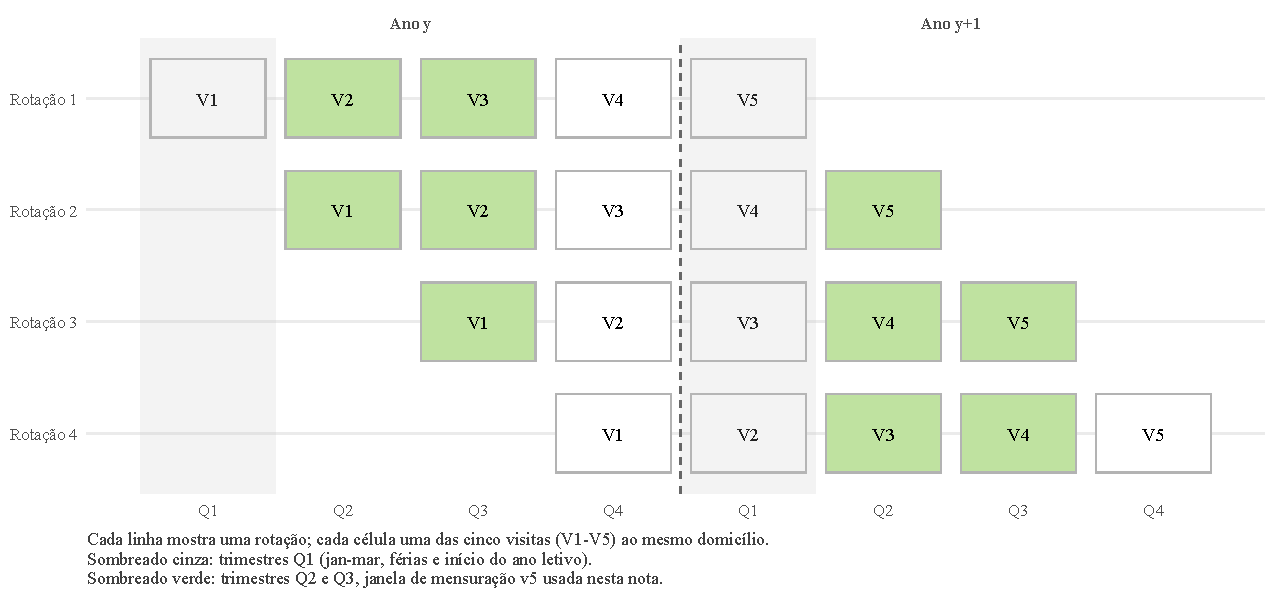
\includegraphics[width=0.95\textwidth]{../DataWork/5_Figures/output/F0_esquema_rotativo.pdf}
\caption{Esquema rotativo 1-2(5) da PNADC e janela de mensuração v5.}
\label{fig:esquema_rotativo}
\figurenote{Cada linha é uma rotação; cada célula é uma das cinco
visitas (V1--V5) ao mesmo domicílio. A faixa cinza marca os
trimestres $Q_1$ (jan-mar), período de férias e início do ano
letivo. A faixa verde marca $Q_2$ e $Q_3$, janela de mensuração v5
adotada nesta nota. Rotação 1 (entra em $Q_1$ do ano $y$) só tem
observação em $Q_1$ de $y+1$, ficando portanto excluída por
construção da medição entre-anos v5.}
\end{figure}

A consequência imediata desse esquema é que, para qualquer
domicílio do painel, sempre existe pelo menos uma observação em
dois anos calendário consecutivos. Em outras palavras, todo
domicílio necessariamente atravessa a virada de ano, o que torna a
PNADC um instrumento naturalmente vocacionado para medir transições
entre anos letivos. Há, contudo, uma assimetria importante.
Independentemente do trimestre de entrada, a primeira observação
no ano $y+1$ ocorre quase sempre no $Q_1$ desse ano. Em termos
práticos, isso significa que, sem ajuste metodológico, mais de
noventa por cento das transições $t \to t+1$ seriam medidas com
observação em $t+1$ em janeiro, fevereiro ou março, exatamente o
período em que o ano letivo brasileiro está em férias ou em sua
fase inicial. Para evitar esse viés, esta nota restringe a janela
de medição entre-anos aos trimestres $Q_2$ e $Q_3$ de cada ano,
indicados em verde na Figura~\ref{fig:esquema_rotativo}.
Domicílios de rotação 1, que não têm nenhuma observação em $Q_2$
ou $Q_3$ do ano $y+1$, são por construção excluídos da medição
entre-anos. A discussão completa do efeito-férias e das alternativas
metodológicas está na Seção~\ref{ssec:efeito_ferias}.

Esse \emph{design} cria duas janelas naturais para medir o fluxo
escolar. A janela intra-ano corresponde à primeira e à última
observação de um mesmo indivíduo dentro de um ano calendário,
separadas tipicamente por dois a quatro trimestres, e captura
saídas da escola que ocorreram dentro do ano letivo, o conceito
operacional de abandono. A janela entre-anos corresponde a uma
observação em $Q_2$ ou $Q_3$ de um ano calendário e a observação
correspondente em $Q_2$ ou $Q_3$ do ano seguinte, e captura
transições entre anos letivos, abrangendo os conceitos de evasão,
promoção, repetência e migração para EJA.

A construção do painel exige duas operações, a saber, a
identificação estável do domicílio entre visitas e a identificação
estável de cada pessoa dentro do domicílio. Construímos o
identificador de domicílio como a concatenação de quatro variáveis,
isto é, unidade federativa (\texttt{UF}), unidade primária de
amostragem (\texttt{UPA}), número de seleção do domicílio dentro
da UPA (\texttt{V1008}) e número do painel (\texttt{V1014}).
Domicílios pertencentes ao mesmo painel são entrevistados nos
mesmos cinco trimestres consecutivos, de modo que a chave
\texttt{UF + UPA + V1008 + V1014} é estável por construção e
identifica o domicílio através das visitas. Dentro de cada
domicílio, a posição da pessoa na lista de moradores é codificada
pela variável \texttt{V2003}. O \emph{matching} preliminar de uma
mesma pessoa entre visitas usa, portanto, a combinação
\texttt{hh\_id + V2003}. Como \texttt{V2003} pode variar caso haja
entrada ou saída de moradores entre visitas, implementamos três
camadas de validação por sexo (\texttt{V2007}), idade (\texttt{V2009})
e reconciliação por correspondência de atributos. Indivíduos com elo
válido em pelo menos duas visitas formam o painel, e as taxas de
\emph{matching} obtidas estão reportadas na
Seção~\ref{ssec:atrito}. Os detalhes operacionais das três camadas
de validação estão no Apêndice~\ref{app:variaveis}.

Os pesos amostrais da PNADC trimestral, codificados na variável
\texttt{V1028}, são calibrados para representatividade trimestral,
e não longitudinal. Para indicadores de fluxo, usamos o peso da
primeira observação do indivíduo no painel, esquema que designamos
por P1. Reportamos um teste de robustez na
Seção~\ref{ssec:atrito} usando reponderação por \emph{inverse
propensity} para corrigir atrito, seguindo a metodologia padrão
de painel rotativo.\footnote{A literatura sobre reponderação em
painéis com atrito foi formalizada por
\citet{wooldridge_2007_attrition} e adaptada para a PNADC em
\citet{IPEA2022_painel}.} Para evitar células com imprecisão
excessiva, suprimimos das tabelas qualquer combinação (subgrupo,
indicador, ano) com $N < 30$. Reportamos $N$ efetivo em todas as
tabelas e o intervalo de confiança \emph{bootstrap}, com
\emph{cluster} em UPA, nas tabelas principais.

\begin{caixatexto}{Caixa 1: Uma família ao longo dos cinco trimestres}
Para fixar ideias, considere a família M., entrevistada pela PNADC
pela primeira vez em 2023Q2 (rotação 2). O domicílio é identificado
pela combinação \texttt{UF=33, UPA=001234567, V1008=05, V1014=02}.
Na primeira visita, o domicílio tem cinco moradores, a saber, o
casal M., com 40 e 38 anos respectivamente, e três filhos, isto é,
Pedro, de 16 anos, no primeiro ano do EM; Maria, de 13 anos, no
oitavo ano do EF; e João, de 7 anos, no segundo ano do EF. Em
2023Q2, Pedro estuda (\texttt{V3002=1}) em escola estadual
(\texttt{V3002A=3}) no primeiro ano do EM (\texttt{V3006=1}). Em
2023Q3, Pedro mantém a mesma série, confirmando a observação. Em
2024Q2 (quinta visita), Pedro tem 17 anos e responde
\texttt{V3002=1} (frequenta) no segundo ano do EM
(\texttt{V3006=2}), tendo sido promovido entre 2023 e 2024.

A linkagem produz duas observações no painel longitudinal. A
primeira é o registro de Pedro em $Q_2$ ou $Q_3$ de 2023 com
nível 10 (1º ano do EM). A segunda é o registro de Pedro em
$Q_2$ de 2024 com nível 11 (2º ano do EM). Como nível em $t+1$ é
superior a nível em $t$, a transição é classificada como
promoção. Se Pedro estivesse, ao invés disso, sem matrícula em
2024Q2 mas com $V3014=1$ (concluiu o curso anterior), seria
classificado como promoção mesmo sem matrícula posterior, em
alinhamento com a definição do INEP para conclusão do EM. E se
ele estivesse frequentando uma escola privada em 2024, apareceria
com $V3002A=1$, ainda contado como promoção, mas com a mudança de
rede pública para privada visível apenas para a PNADC, não para
o Censo Escolar. Essa é a essência da captura de retorno.
\end{caixatexto}

\subsection{Harmonização de variáveis educacionais}

A PNADC mudou o nome e o significado dos códigos de algumas
variáveis educacionais em 2016. Especificamente, na variável
\texttt{V3003} pré-2016, o código 3 representava ``Regular
Fundamental'', o código 5 ``Regular Médio'' e o código 7
``Educação Profissional Médio'', enquanto na variável
\texttt{V3003A} pós-2016, os mesmos conceitos são representados
pelos códigos 4, 6 e 7, respectivamente. Esta nota harmoniza as
duas codificações em \texttt{etapa\_consolid}, conforme detalhado
no Apêndice~\ref{app:variaveis}. A Tabela~\ref{tab:harmonizacao}
resume o mapeamento das principais variáveis entre as duas versões.

\begin{table}[htbp]
\centering
\caption{Harmonização de variáveis educacionais entre versões da PNADC}
\label{tab:harmonizacao}
\begin{tabular}{lll}
\toprule
Conceito                                 & Versão pré-2016 & Versão 2016+    \\
\midrule
Frequenta escola                         & V3002           & V3002           \\
Rede da escola                           & V3002A          & V3002A          \\
Curso/etapa que frequenta                & V3003 (códigos 3, 5, 7) & V3003A (códigos 4, 6, 7) \\
Série/ano que frequenta                  & V3006 & V3006 \\
Concluiu o curso? (último frequentado)   & V3014 & V3014 \\
Último ano/série concluído               & V3013 & V3013A \\
\bottomrule
\end{tabular}
\end{table}

Na harmonização, \texttt{etapa\_consolid} consolida o curso em
códigos uniformes para todo o período. Da \texttt{etapa\_consolid}
e da \texttt{V3006}, derivamos a variável de \emph{nível}, um
índice ordinal monotônico que combina etapa e série. Valores de
um a cinco correspondem aos anos do EF iniciais, seis a nove aos
anos do EF finais, dez a doze aos três anos do EM regular, e
treze ao quarto ano do EM técnico, que existe em parte dos cursos
de educação profissional integrada. A macroetapa, derivada do
nível, distingue EF iniciais (níveis 1 a 5), EF finais (níveis 6
a 9) e Ensino Médio (níveis 10 a 13, regular ou técnico). EJA EF
e EJA EM são tratadas como modalidades separadas, fora do painel
principal mas reportadas em apêndice.

\subsection{Definições operacionais dos cinco indicadores}
\label{ssec:definicoes}

Os cinco indicadores são, em palavras, os seguintes. O abandono é
a fração de alunos matriculados em regular EF ou EM regular ou
técnico na primeira observação do ano $t$ que apresenta
$\text{freq}=0$ na última observação do mesmo ano $t$. Mudança
de modalidade dentro do ano, especificamente do EM regular para
EJA, é tratada como migração para EJA intra-ano, não como
abandono. A migração para EJA entre-anos é a fração que migra
para EJA EF ou EJA EM entre $t$ e $t+1$. A evasão entre-anos é a
fração que não está matriculada em $t+1$ e não migrou para EJA. A
promoção entre-anos é a fração com nível em $t+1$ estritamente
superior ao nível em $t$. A repetência entre-anos é a fração com
nível em $t+1$ igual ao nível em $t$, na mesma etapa.

Para o cálculo das taxas entre-anos, a observação de referência em
$t$ é tomada como aquela com o maior nível educacional declarado
entre $Q_2$ e $Q_3$ de $t$; análogo critério se aplica a $t+1$. O
uso de $\max(\text{nível})$ em $t+1$ protege contra o caso em que
a família reporta a série anterior em $Q_2$ e a série nova em
$Q_3$. Adicionalmente, alunos no terceiro ano do EM regular
(nível 12) ou no quarto ano do EM técnico (nível 13) em $t$ que
reportam $\texttt{V3014}=1$ (concluiu o curso) em $t+1$ são
classificados como promoção, mesmo sem matrícula posterior, em
alinhamento com a definição operacional do INEP. Para a janela
intra-ano, a amostra é restrita a alunos com observações em pelo
menos dois trimestres do mesmo ano, com a primeira observação em
EF ou EM regular ou técnico. As fórmulas matemáticas explícitas
de cada indicador estão no Apêndice~\ref{app:variaveis}.

A diferença metodológica entre o PROFLUXO e a abordagem desta nota
é substantiva. A Tabela~\ref{tab:contraste_profluxo} sintetiza as
principais dimensões. Em essência, o PROFLUXO usa um modelo para
identificar fluxos não observáveis, ao passo que a PNADC longitudinal
substitui o modelo por observação. O custo da nova abordagem é a
dependência da hipótese de que o atrito do painel seja
\emph{ignorable}, condição que testamos diretamente na
Seção~\ref{sec:robustez}.

\begin{table}[htbp]
\centering
\caption{Contraste técnico: PROFLUXO vs. PNADC longitudinal}
\label{tab:contraste_profluxo}
\small
\begin{tabular}{p{4cm} p{5cm} p{5cm}}
\toprule
Dimensão            & PROFLUXO (Fletcher-Ribeiro-Klein)            & PNADC longitudinal (esta nota)              \\
\midrule
Dado fundamental    & Matriz idade-série de um corte da PNAD       & Pares ($t$, $t+1$) do mesmo indivíduo       \\
Identificação       & Modelo de fluxo estacionário                 & Observação direta                            \\
Hipóteses fortes    & Estacionariedade; transições homogêneas      & Atrito ignorable (testável)                  \\
Heterogeneidade fina& Limitada (requer rodar modelo por subgrupo)  & Direta (média ponderada por subgrupo)        \\
Choques estruturais & Indistinguíveis no curto prazo               & Detectáveis em janela trimestral             \\
Mudança de canal    & Difícil de incorporar (modelo é fechado)     & Direta (mudança de rede é observável)        \\
Tempo de implementação & Lento (caderno de modelagem por ciclo)    & Reprodutível em código                       \\
\bottomrule
\end{tabular}
\end{table}

A análise de heterogeneidade da Seção~\ref{sec:heterogeneidade}
mobiliza um conjunto de variáveis de estratificação que merece
descrição. A defasagem idade-série é calculada com base na
convenção de entrada aos seis anos no primeiro ano do EF e
classifica os alunos em três categorias, isto é, em dia, quando a
idade é menor ou igual à idade-padrão, um ano defasado e dois ou
mais anos defasados. O sexo é registrado pela variável
\texttt{V2007} e a raça/cor pela \texttt{V2010}, que distingue as
categorias branca, preta, parda, amarela e indígena. Os quintis
nacionais de renda domiciliar per capita são computados anualmente
a partir de \texttt{VD5008}, ponderados pelo peso amostral, e
construídos em base nacional, não por UF. O perfil de elegibilidade
ao Bolsa Família é definido como renda domiciliar per capita
menor ou igual a meio salário-mínimo no ano, limiar que é uma
aproximação à elegibilidade ao Programa Bolsa Família, ao Auxílio
Brasil e ao CadÚnico. Adicionalmente, em uma subamostra
correspondente à quinta visita da PNADC anual, com seu suplemento
de Programas Sociais, dispomos da variável \texttt{V5002A}, que
indica diretamente se o domicílio recebe Bolsa Família, e essa
subamostra cobre aproximadamente vinte por cento das transições
do painel. A rede é categorizada como pública, englobando federal,
estadual e municipal, ou privada, conforme a variável
\texttt{V3002A}. Por fim, a macrorregião classifica o domicílio
em Norte, Nordeste, Sudeste, Sul ou Centro-Oeste. Cabe uma nota
sobre a relação dessas variáveis com o CadÚnico. A PNADC não tem
variável direta de inscrição no Cadastro Único. Quem recebe Bolsa
Família é, por construção, cadastrado, mas a recíproca não é
verdadeira, pois famílias inscritas no CadÚnico que não recebem o
benefício por estarem acima da linha do programa não são
identificáveis diretamente. Reportamos, portanto, resultados pelo
perfil de elegibilidade, com renda domiciliar per capita menor ou
igual a meio salário-mínimo, enfatizando que se trata de uma
aproximação.

% =========================================================================
% Secao 4 - Resultados agregados Brasil
% =========================================================================

\section{Resultados agregados para o Brasil}
\label{sec:agregados}

A Tabela~\ref{tab:t1_brasil} reporta os indicadores de fluxo escolar
para o Brasil, por macroetapa e ano calendário, no período
2012--2023. As taxas inter-ano são calculadas com a metodologia
descrita na Seção~\ref{ssec:definicoes}, em que a observação de
referência em $t$ e em $t+1$ é tomada entre os trimestres $Q_2$ e
$Q_3$ de cada ano, usando o máximo do nível educacional declarado.
A taxa de abandono é calculada na subamostra dos alunos com
observação nos quatro trimestres do mesmo ano e é reportada
separadamente na Tabela~\ref{tab:abandono_fullyear}.

% Auto-gerado por C17_correcao_em_concluido.py - versao v3 (com correcao EM concluido)
\begin{table}[htbp]
\centering
\caption{Indicadores agregados de fluxo escolar, Brasil, por macroetapa e ano. Painel longitudinal da PNADC, 2012--2023, com corre\c{c}\~ao de EM conclu\'ido via \texttt{V3014}.}
\label{tab:t1_brasil}
\begin{threeparttable}
\small
\begin{tabular}{lrrrrrr}
\toprule
Ano & Promo\c{c}\~ao & Repet\^encia & Evas\~ao & Migra\c{c}\~ao EJA & Abandono$^{a}$ & N \\
    & (\%)            & (\%)        & (\%)     & (\%)               & (\%)            &   \\
\midrule
\multicolumn{7}{l}{\textit{Painel A: EF iniciais (1\textsuperscript{o}--5\textsuperscript{o} ano)}} \\
\midrule
2012 & 77.3 & 17.0 & 1.1 & 0.3 & 1.7 & 13.651 \\
2013 & 78.8 & 15.9 & 1.0 & 0.2 & 1.4 & 12.364 \\
2014 & 80.7 & 14.7 & 0.8 & 0.1 & 0.9 & 12.343 \\
2015 & 80.5 & 15.5 & 0.6 & 0.2 & 0.6 & 13.151 \\
2016 & 82.3 & 14.3 & 0.5 & 0.2 & 0.5 & 13.105 \\
2017 & 84.9 & 12.6 & 0.6 & 0.2 & 0.6 & 12.721 \\
2018 & 85.7 & 11.6 & 0.4 & 0.3 & 0.7 & 12.424 \\
2019 & 85.5 & 11.8 & 0.4 & 0.1 & 0.5 & 10.055 \\
2020$^{\dagger}$ & 75.8 & 21.6 & 0.4 & 0.0 & 0.7 & 6.357 \\
2021$^{\dagger}$ & 82.1 & 15.8 & 0.2 & 0.1 & 0.3 & 8.088 \\
2022 & 73.0 & 25.4 & 0.1 & 0.0 & 0.2 & 9.629 \\
2023 & 72.4 & 26.1 & 0.3 & 0.0 & 0.2 & 10.164 \\
\\[0.3em]
\multicolumn{7}{l}{\textit{Painel B: EF finais (6\textsuperscript{o}--9\textsuperscript{o} ano)}} \\
\midrule
2012 & 73.6 & 15.9 & 3.2 & 1.5 & 4.1 & 10.375 \\
2013 & 73.9 & 16.6 & 3.2 & 1.4 & 3.4 & 9.790 \\
2014 & 76.2 & 16.1 & 2.7 & 0.9 & 3.7 & 9.865 \\
2015 & 76.3 & 16.1 & 2.4 & 1.5 & 2.7 & 10.447 \\
2016 & 77.5 & 15.1 & 2.1 & 1.5 & 2.6 & 10.699 \\
2017 & 78.7 & 14.9 & 2.0 & 1.5 & 2.5 & 10.553 \\
2018 & 80.2 & 13.4 & 2.1 & 1.9 & 2.1 & 10.110 \\
2019 & 81.1 & 13.8 & 1.3 & 0.8 & 2.2 & 8.468 \\
2020$^{\dagger}$ & 72.9 & 24.5 & 0.8 & 0.5 & 0.6 & 5.424 \\
2021$^{\dagger}$ & 80.3 & 15.9 & 2.0 & 0.4 & 0.8 & 7.463 \\
2022 & 71.2 & 25.9 & 1.3 & 0.4 & 0.9 & 8.172 \\
2023 & 70.1 & 27.6 & 0.9 & 0.4 & 0.5 & 8.624 \\
\\[0.3em]
\multicolumn{7}{l}{\textit{Painel C: Ensino M\'edio (1\textsuperscript{o}--3\textsuperscript{o} ano)}} \\
\midrule
2012 & 65.8 & 14.4 & 7.1 & 1.1 & 15.2 & 6.672 \\
2013 & 65.5 & 14.8 & 7.7 & 0.9 & 13.5 & 6.260 \\
2014 & 67.2 & 15.6 & 6.6 & 1.2 & 12.8 & 6.518 \\
2015 & 65.2 & 16.7 & 6.0 & 1.6 & 12.9 & 6.978 \\
2016 & 68.0 & 14.8 & 5.8 & 2.2 & 11.3 & 7.293 \\
2017 & 69.6 & 12.7 & 5.7 & 2.6 & 14.1 & 6.706 \\
2018 & 71.0 & 12.0 & 5.8 & 2.0 & 13.0 & 6.678 \\
2019 & 70.7 & 13.4 & 4.9 & 1.3 & 12.8 & 5.692 \\
2020$^{\dagger}$ & 61.7 & 28.8 & 3.0 & 0.8 & 3.2 & 3.541 \\
2021$^{\dagger}$ & 70.1 & 16.5 & 5.7 & 1.1 & 8.7 & 4.815 \\
2022 & 61.7 & 25.3 & 4.4 & 0.5 & 9.1 & 5.473 \\
2023 & 61.1 & 26.4 & 4.3 & 0.5 & 7.7 & 5.536 \\
\bottomrule
\end{tabular}
\begin{tablenotes}\footnotesize
\item \textit{Fonte:} Painel longitudinal da PNADC trimestral (IBGE), 2012Q1--2024Q4.
\item \textit{Notas:} Refer\^encia em $t$ e $t+1$ tomada entre $Q_2$ e $Q_3$, com $\max(\text{n\'ivel})$ em $t+1$. Alunos no terceiro ano do EM em $t$ que reportam $\texttt{V3014}=1$ (concluiu o curso) em $t+1$ s\~ao classificados como promo\c{c}\~ao, mesmo com $\texttt{V3002}=2$ em $t+1$, em alinhamento com a defini\c{c}\~ao do INEP. Abandono \'e a m\'edia da Tabela~\ref{tab:abandono_fullyear}.
\item $^{a}$Abandono refere-se \`a taxa intra-ano da Tabela~\ref{tab:abandono_fullyear}.
\item $^{\dagger}$Anos afetados pela pandemia COVID-19.
\item \emph{N} \'e o n\'umero de transi\c{c}\~oes individuais (n\~ao ponderado). Taxas ponderadas pelo peso amostral $w_i^{P1}$.
\end{tablenotes}
\end{threeparttable}
\end{table}


Três achados são imediatos na Tabela~\ref{tab:t1_brasil}. Em primeiro
lugar, a taxa de promoção é alta no EF iniciais e mais baixa no EM,
padrão consistente com o gargalo histórico do ensino médio
brasileiro. Em 2019, a promoção é de 85,5\% no EF iniciais, 81,1\%
no EF finais e 50,4\% no EM, e a soma de promoção, repetência,
evasão e migração para EJA é de 97,8\% no EF iniciais, 97,0\% no
EF finais e 90,3\% no EM. Em segundo lugar, a evasão concentra-se
quase exclusivamente no EM. Em 2019, a evasão entre anos é de 0,4\%
no EF iniciais, 1,3\% no EF finais e 25,3\% no EM, salto que define
o EM brasileiro como ponto crítico do sistema. Em terceiro lugar, o
diferencial de promoção entre EF iniciais e EM, da ordem de trinta e
cinco pontos percentuais, reproduz, com nova metodologia e janela
contemporânea, o padrão histórico identificado pela literatura
brasileira desde \citet{Ribeiro1991_pedagogia}, em que a transição
do EF para o EM funciona como funil restritivo.

A Tabela~\ref{tab:abandono_fullyear} reporta a taxa de abandono
intra-ano. Em 2019, o abandono é de apenas 0,5\% no EF iniciais,
2,2\% no EF finais e 12,8\% no EM. A diferença entre as três
macroetapas é nítida, refletindo a mesma estrutura que aparece na
evasão entre anos. O abandono no EM em 2019, da ordem de treze por
cento, é mais de seis vezes maior do que no EF finais e mais de
vinte vezes maior do que no EF iniciais.

% C30b - abandono v5 corrected (V3014 aplicada)
\begin{table}[htbp]
\centering
\caption{Taxa de abandono intra-ano (cobertura completa Q1--Q4) com corre\c{c}\~ao \texttt{V3014} para conclus\~ao terminal do EM, Brasil, 2012--2024.}
\label{tab:abandono_fullyear}
\begin{threeparttable}
\small
\begin{tabular}{lrrr}
\toprule
Ano & Abandono (\%) & Migra\c{c}\~ao EJA intra-ano (\%) & N \\
\midrule
\multicolumn{4}{l}{\textit{EF iniciais}} \\
\midrule
2012 & 1.7 & 0.1 & 12.521 \\
2013 & 1.4 & 0.1 & 10.703 \\
2014 & 0.9 & 0.1 & 10.890 \\
2015 & 0.6 & 0.0 & 11.084 \\
2016 & 0.5 & 0.1 & 12.121 \\
2017 & 0.6 & 0.1 & 11.964 \\
2018 & 0.7 & 0.1 & 11.510 \\
2019 & 0.5 & 0.1 & 11.023 \\
2020$^{\dagger}$ & 0.6 & 0.0 & 7.148 \\
2021$^{\dagger}$ & 0.3 & 0.1 & 4.601 \\
2022 & 0.2 & 0.0 & 8.549 \\
2023 & 0.2 & 0.0 & 8.457 \\
2024 & 0.4 & 0.0 & 8.975 \\
\\[0.3em]
\multicolumn{4}{l}{\textit{EF finais}} \\
\midrule
2012 & 4.0 & 1.0 & 9.302 \\
2013 & 3.4 & 0.7 & 8.677 \\
2014 & 3.6 & 0.7 & 8.855 \\
2015 & 2.7 & 0.0 & 9.011 \\
2016 & 2.5 & 1.3 & 10.259 \\
2017 & 2.4 & 0.8 & 10.180 \\
2018 & 2.1 & 0.9 & 9.562 \\
2019 & 2.2 & 0.8 & 9.407 \\
2020$^{\dagger}$ & 0.6 & 0.2 & 6.195 \\
2021$^{\dagger}$ & 0.8 & 0.1 & 4.399 \\
2022 & 0.9 & 0.2 & 7.860 \\
2023 & 0.5 & 0.3 & 7.465 \\
2024 & 1.5 & 0.6 & 7.704 \\
\\[0.3em]
\multicolumn{4}{l}{\textit{EM}} \\
\midrule
2012 & 7.9 & 1.0 & 6.161 \\
2013 & 6.8 & 0.8 & 5.766 \\
2014 & 5.9 & 0.6 & 6.170 \\
2015 & 6.2 & 0.0 & 6.055 \\
2016 & 5.4 & 1.2 & 6.976 \\
2017 & 6.7 & 1.5 & 6.927 \\
2018 & 5.7 & 1.5 & 6.304 \\
2019 & 5.8 & 1.6 & 6.182 \\
2020$^{\dagger}$ & 1.7 & 0.7 & 4.194 \\
2021$^{\dagger}$ & 2.3 & 0.4 & 3.084 \\
2022 & 3.8 & 0.4 & 5.160 \\
2023 & 2.5 & 0.5 & 5.164 \\
2024 & 5.2 & 0.9 & 5.254 \\
\bottomrule
\end{tabular}
\begin{tablenotes}\footnotesize
\item \textit{Fonte:} Painel longitudinal da PNADC.
\item \textit{Notas:} Subamostra restrita aos alunos com observa\c{c}\~oes em todos os quatro trimestres do mesmo ano (\emph{rota\c{c}\~ao 1}). Abandono \'e definido como \texttt{V3002=1} em Q1 e \texttt{V3002=0} em Q4 do mesmo ano, \emph{exceto} para alunos no terceiro ano do EM regular ou no quarto ano do EM t\'ecnico (\emph{n\'ivel}~12--13) cuja \texttt{V3014=1} em alguma observa\c{c}\~ao do ano (conclus\~ao terminal). Esses s\~ao reclassificados como conclus\~ao, n\~ao abandono.
\item $^{\dagger}$Anos afetados pela pandemia COVID-19.
\end{tablenotes}
\end{threeparttable}
\end{table}


A Figura~\ref{fig:freq_trimestre} mostra o percentual de alunos
frequentando a escola ao longo dos quatro trimestres do ano, por
macroetapa, em anos selecionados. No EF iniciais e finais, o
percentual de frequência fica próximo de cem por cento ao longo de
todos os trimestres, com leve queda em $Q_4$, sinalizando o
encerramento do ano letivo e o início das férias. No EM, a queda em
$Q_4$ é mais pronunciada, em torno de quatro a oito pontos
percentuais, evidência da saída de alunos antes do encerramento do
ano letivo.

\begin{figure}[htbp]
\centering
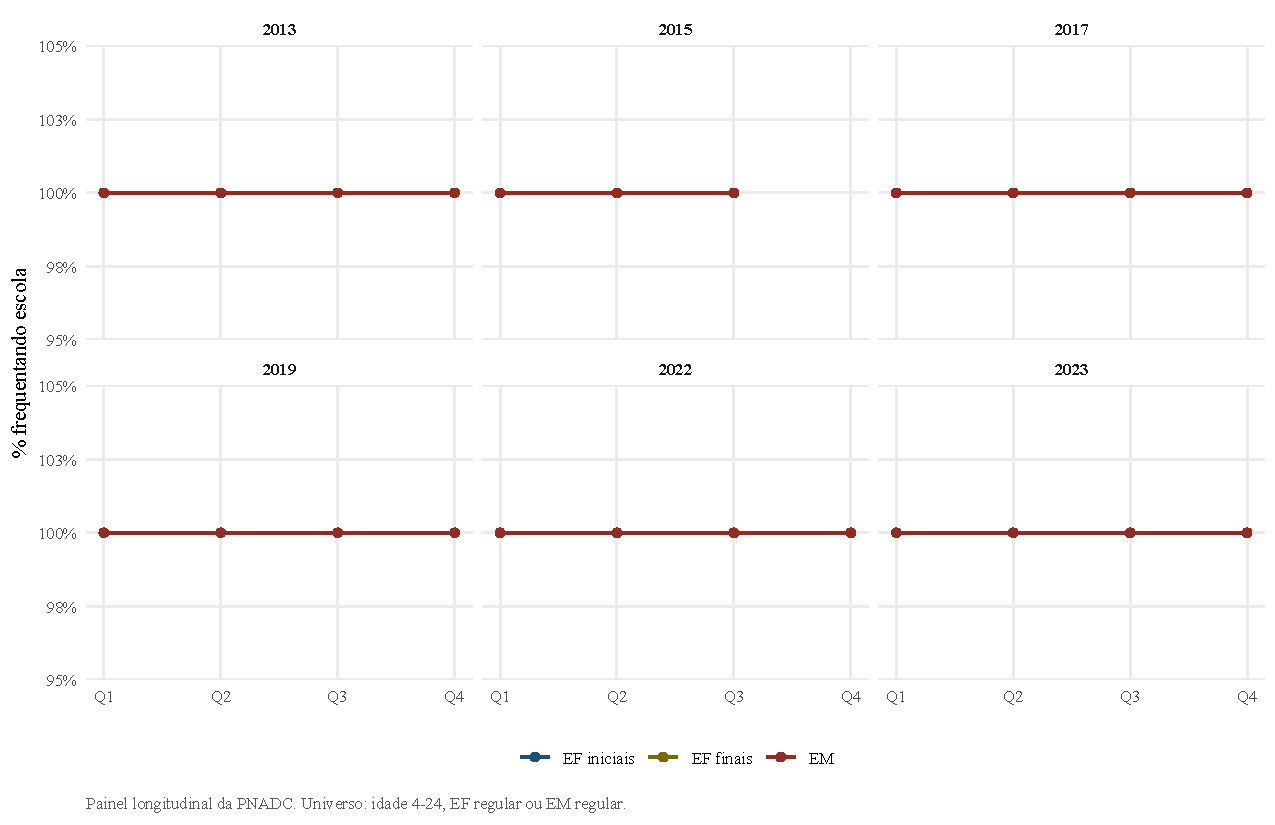
\includegraphics[width=0.95\textwidth]{../DataWork/5_Figures/output/F7_freq_por_trimestre.pdf}
\caption{Percentual de alunos frequentando escola por trimestre, por
macroetapa, anos selecionados.}
\label{fig:freq_trimestre}
\figurenote{Universo: idade quatro a vinte e quatro anos no painel
PNADC, em EF regular ou EM regular. O percentual de frequência é
calculado dentro de cada combinação $($Ano, Trimestre, macroetapa$)$
ponderado pelo peso amostral.}
\end{figure}

A Figura~\ref{fig:cohort_fluxo} replica, com dados da PNADC
trimestral, o exercício de \citet{Fernandes2011_atratividade},
originalmente realizado com dados mensais da PME. Mostramos o índice
de matrículas, normalizado a cem no início de cada série, ao longo
de dezesseis trimestres, para pseudocoortes que entram no oitavo ano
do EF em diferentes anos calendário e progridem até o terceiro ano
do EM. As linhas verticais tracejadas marcam as transições entre
séries, em janeiro do ano seguinte. O Painel A considera todos os
alunos, enquanto o Painel B restringe a alunos sem distorção
idade-série.

\begin{figure}[htbp]
\centering
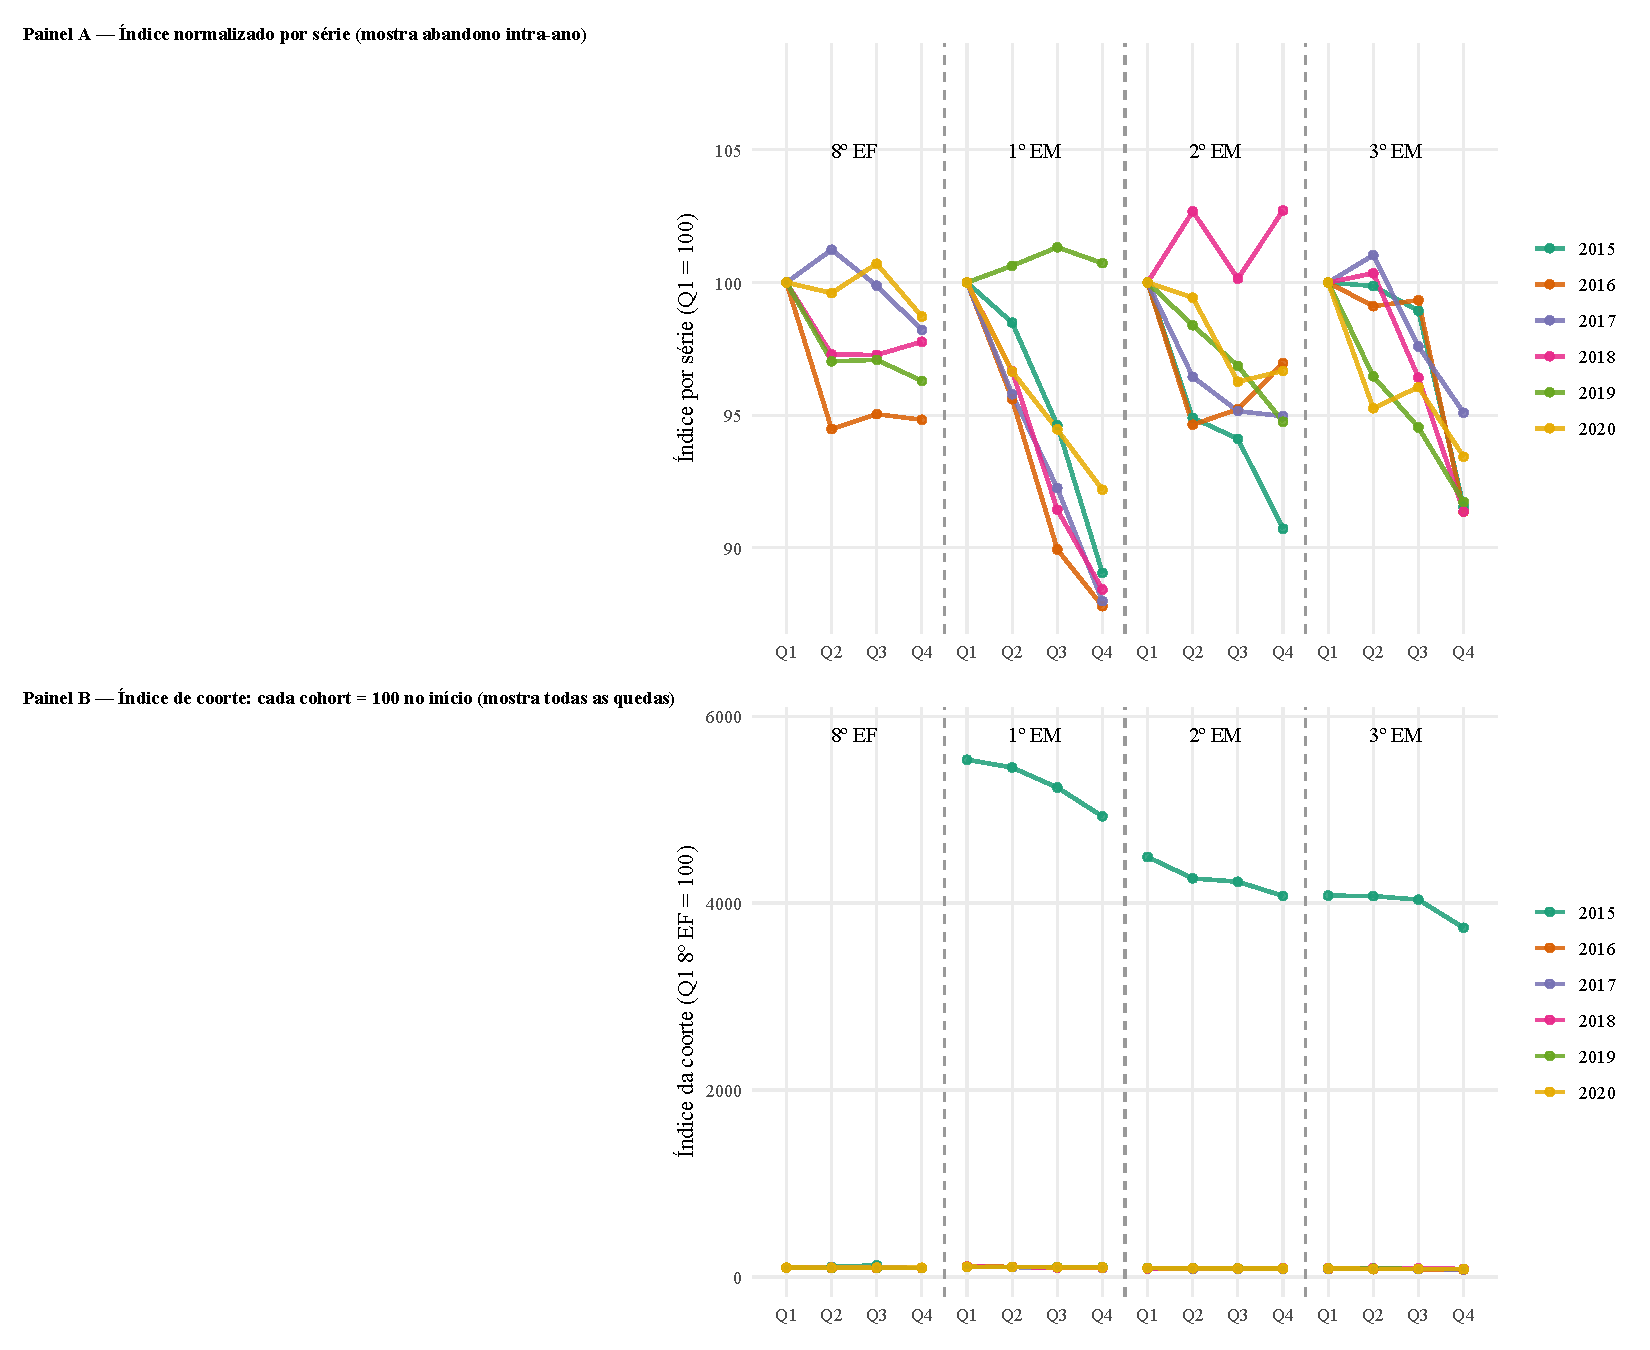
\includegraphics[width=0.95\textwidth]{../DataWork/5_Figures/output/F4_cohort_fluxo.pdf}
\caption{Índice de matrículas por trimestre, ao longo de pseudocoortes
oitavo EF $\to$ terceiro EM (PNADC trimestral, 2013--2024).}
\label{fig:cohort_fluxo}
\figurenote{Cada coorte é definida pela combinação de série-base e
ano calendário de entrada no oitavo EF. O Painel A, com normalização
por série, isto é, cem em $Q_1$ de cada série, evidencia o padrão de
abandono intra-ano. O Painel B, com normalização por coorte, ou seja,
cem em $Q_1$ do oitavo EF, revela todas as quedas, intra-ano
(abandono) e entre séries (evasão, repetência e migração para EJA).
Reproduz e estende o exercício de \citet{Fernandes2011_atratividade}.}
\end{figure}

Três padrões emergem da figura. Em primeiro lugar, no Painel A, a
queda intra-ano dentro de cada série é modesta no oitavo EF e
amplifica-se progressivamente no ensino médio, confirmando o padrão
documentado por \citet{Fernandes2011_atratividade}, em que o
abandono cresce com a idade e com a série. Em segundo lugar, no
Painel B, fica visível que a maior parte da atrição ocorre nas
transições entre séries, isto é, nos saltos verticais nas linhas
tracejadas, e não dentro de cada ano, padrão consistente com o
gargalo histórico do ensino médio brasileiro
\citep{Klein2006_educacao, IMDS_PereiraA002}. Por fim, em terceiro
lugar, ao final dos dezesseis trimestres, o índice da coorte
(Painel B) está em torno de 40\% a 60\% do nível inicial, dependendo
da coorte. Ou seja, apenas cerca de metade dos alunos que estavam no
oitavo EF chegam ao terceiro EM três anos depois, diagnóstico que
motiva a agenda de políticas focalizadas como o Pé-de-Meia
\citep{Brasil2024_PeDeMeia}.

Entre 2012 e 2019, observa-se melhoria consistente em todos os
indicadores do EF. A promoção no EF iniciais sobe de 77,3\% em 2012
para 85,5\% em 2019, e a repetência cai de 17,0\% para 11,8\%. No
EM, a promoção cresce mais modestamente, de 47,6\% em 2012 para
50,4\% em 2019, com a evasão estável em torno de 24\% a 26\%. A
pandemia de COVID-19 interrompe a melhoria. Em 2020, no EF iniciais,
a promoção cai abruptamente para 75,8\% e a repetência sobe para
21,6\%, inversão dramática provavelmente associada às políticas de
aprovação automática ou de suspensão da aprovação adotadas de modo
heterogêneo entre estados e municípios durante a suspensão de aulas
presenciais. Os números de 2020 e 2021 não devem ser interpretados
como piora real do aprendizado, pois refletem rupturas
administrativas no conceito de aprovação. A partir de 2022, observa-se
retomada parcial, mas os níveis de promoção do EF iniciais em 2023
(72,4\%) ainda não retornaram ao patamar pré-pandemia.

O ano de 2024 marca a entrada do Pé-de-Meia
\citep{Brasil2024_PeDeMeia} no calendário escolar, com pagamento a
partir de março. A medida visa, entre outros objetivos, reduzir a
evasão no EM público. Como o programa só começa em 2024, ainda é
cedo para identificar seus efeitos com a janela do painel da PNADC,
pois a transição 2024--2025 ainda não está disponível. A
monitorização desse impacto será imediatamente possível assim que o
IBGE disponibilizar a PNADC 2025Q1. Os anos de 2020 e 2021 são
tratados separadamente nas tabelas e figuras por duas razões. Em
primeiro lugar, o IBGE conduziu parte das entrevistas por telefone
durante o pico da pandemia, o que pode introduzir viés de
não-resposta diferencial. Em segundo lugar, o fechamento de escolas
reduziu a comparabilidade do conceito de frequentar escola, uma vez
que alunos podiam estar matriculados mas sem aulas presenciais. Nas
figuras, o intervalo 2020--2021 aparece sombreado, e nas tabelas
esses anos vêm marcados com $\dagger$. As séries de média multianual
reportadas na Seção~\ref{sec:heterogeneidade} excluem 2020 e 2021 do
cálculo da média 2018--2023, restringindo-se aos anos pré-COVID
(2018 e 2019) e pós-COVID (2022 e 2023).

% =========================================================================
% Secao 5 - Heterogeneidade socioeconomica
% =========================================================================

\section{Heterogeneidade socioeconômica}
\label{sec:heterogeneidade}

Esta seção explora as desagregações que são, à data desta nota,
inviáveis com os dados publicados pelo INEP, pois o Censo Escolar
não tem renda domiciliar nem raça do aluno individualizada nas
tabelas agregadas oficialmente divulgadas. Os números desta seção
referem-se à média 2018--2023, excluindo 2020 e 2021 para evitar o
ruído COVID, no painel inter-ano da PNADC sob a metodologia v5
descrita na Seção~\ref{ssec:definicoes}. A
Figura~\ref{fig:heterog_combined} consolida as desagregações por
sexo, raça, quintil de renda e defasagem idade-série, em quatro
painéis. Discutimos a seguir os achados centrais. Tabelas
desagregadas detalhadas estão no Apêndice~\ref{app:uf}, e figuras
adicionais nas Figuras~\ref{fig:het_sexo}--\ref{fig:het_regiao}.

\begin{figure}[htbp]
\centering
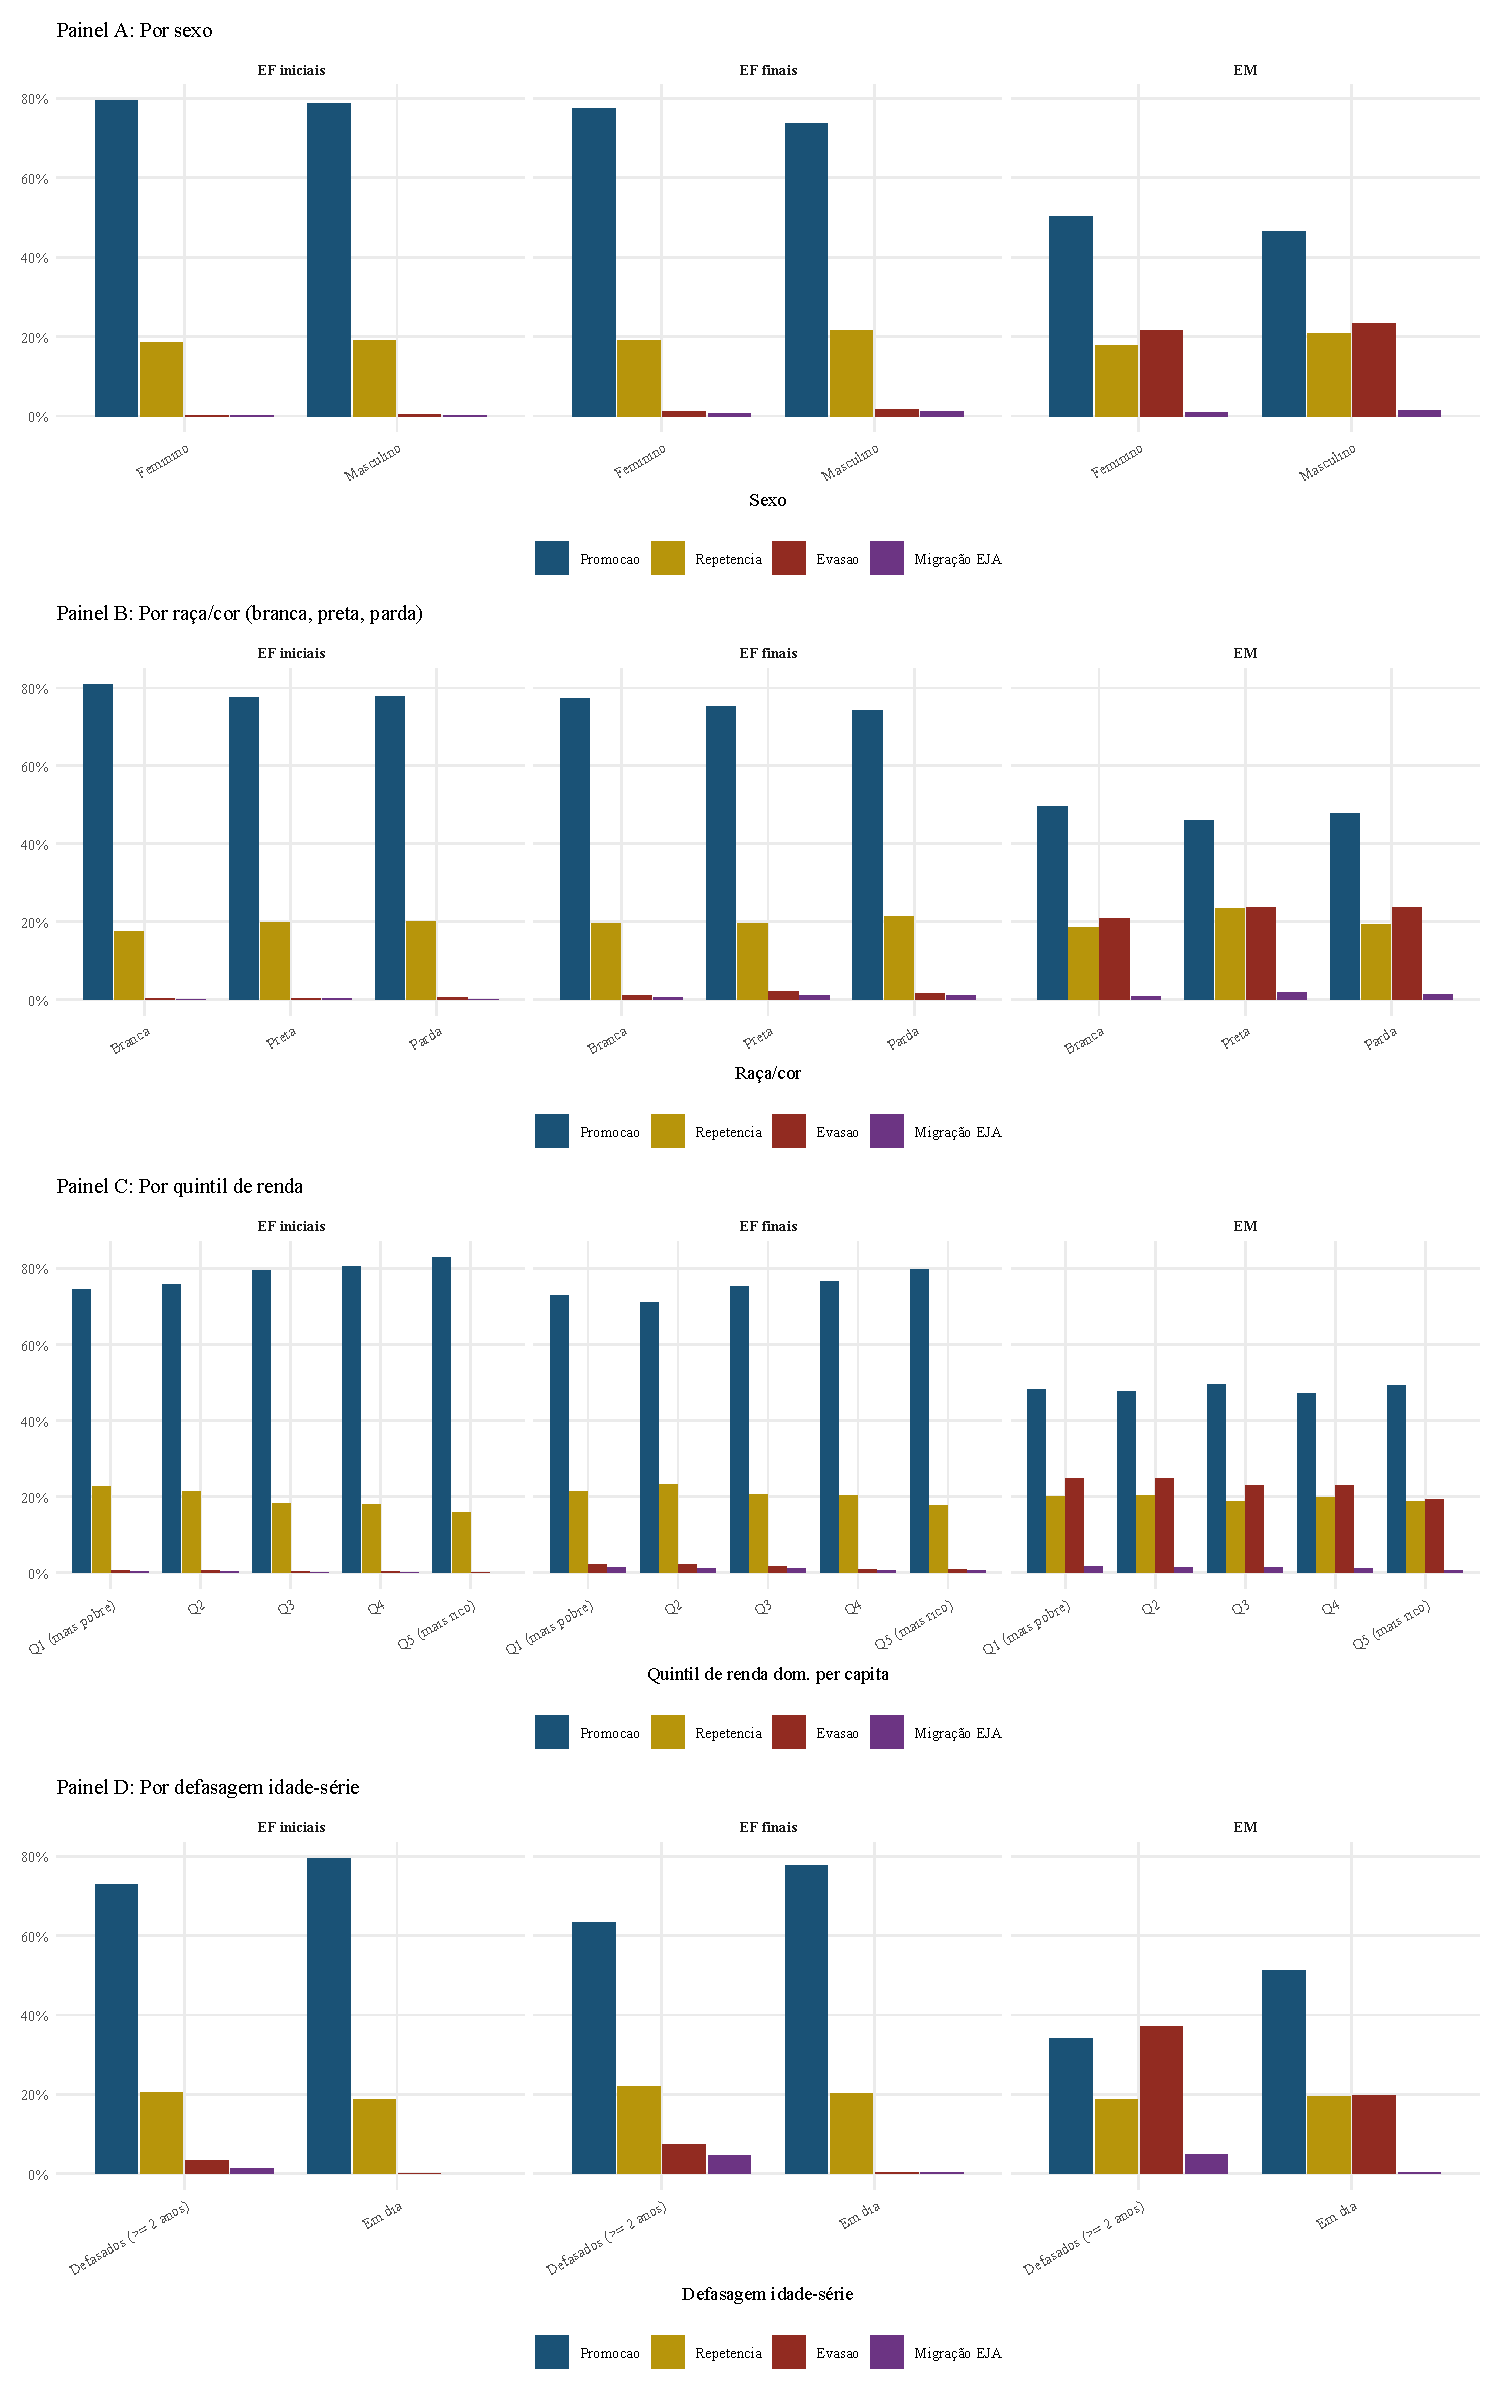
\includegraphics[width=0.95\textwidth]{../DataWork/5_Figures/output/F8_heterog_combined.pdf}
\caption{Taxas de fluxo escolar por dimensão socioeconômica, Brasil,
média 2018--2023 (ex-COVID).}
\label{fig:heterog_combined}
\figurenote{Universo: painel inter-ano da PNADC, com referência em
$t$ e $t+1$ tomadas entre $Q_2$ e $Q_3$ usando o máximo do nível
educacional. Cada painel reporta as quatro taxas (promoção,
repetência, evasão, migração para EJA) por dimensão.}
\end{figure}

A defasagem idade-série é o preditor mais forte de fluxo escolar
desfavorável no painel. A tabela detalhada
(Tabela~\ref{tab:distorcao}, no Apêndice~\ref{app:uf}) reporta as
taxas condicionais ao aluno iniciar o painel com defasagem de
pelo menos dois anos em relação à idade-padrão, comparadas às
taxas dos alunos em dia. As diferenças são substanciais. No EF
iniciais, os alunos defasados têm promoção de 73,0\%, contra
79,5\% dos alunos em dia, e evasão de 3,3\%, contra 0,1\%. No EF
finais, a promoção cai de 77,6\% para 63,2\%, e a evasão sobe de
0,4\% para 7,3\%. No EM, a diferença é dramática. A promoção cai
de 51,2\% para 34,0\%, e a evasão sobe de 19,6\% para 37,1\%, ou
seja, quase o dobro. A taxa de migração para EJA também cresce
muito entre os defasados, chegando a 4,9\% no EM, contra 0,3\%
para alunos em dia. Esse achado replica diretamente o padrão
documentado por \citet{Fernandes2011_atratividade} usando dados
mensais da PME, em que o abandono escolar concentra-se
desproporcionalmente entre alunos defasados, e estende-o ao
período contemporâneo com cobertura nacional. O resultado também
dialoga com \citet{SoaresAlvesFonseca2021_trajetorias} sobre o
uso de trajetórias educacionais como medida agregada de qualidade
da educação básica e com \citet{AlvesSoares2013_contexto} sobre
desigualdades de contexto na efetivação das políticas
educacionais.

Mulheres apresentam consistentemente melhor desempenho em todos os
indicadores e em todas as macroetapas, em linha com a literatura.
A diferença é especialmente visível no EM, em que a promoção
feminina é de cerca de cinquenta e dois por cento contra cinquenta
por cento masculina, com repetência menor entre as mulheres e
evasão similar entre os sexos. O Painel A da
Figura~\ref{fig:heterog_combined} e a Figura~\ref{fig:het_sexo}
detalham esse padrão. Os fatores que levam à evasão no EM
brasileiro afetam ambos os sexos similarmente, mas a vantagem
feminina na progressão de série persiste.

\begin{figure}[htbp]
\centering
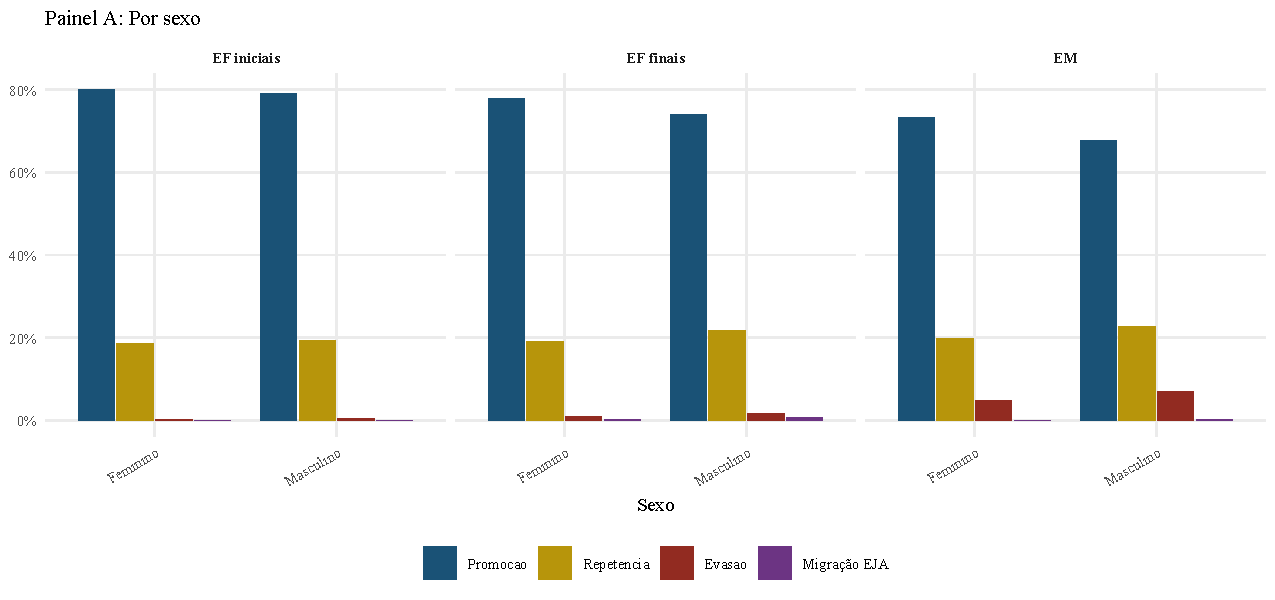
\includegraphics[width=0.95\textwidth]{../DataWork/5_Figures/output/F8a_heterog_sexo.pdf}
\caption{Taxas de fluxo escolar por sexo e macroetapa, média
2018--2023 (ex-COVID).}
\label{fig:het_sexo}
\end{figure}

O gradiente racial é consistente com a literatura recente de
estratificação educacional brasileira. Alunos pretos e pardos
apresentam promoção menor e evasão maior do que alunos brancos
em todas as macroetapas, com a diferença mais pronunciada no EM.
A Figura~\ref{fig:het_raca} reporta as quatro taxas por categoria
racial.

\begin{figure}[htbp]
\centering
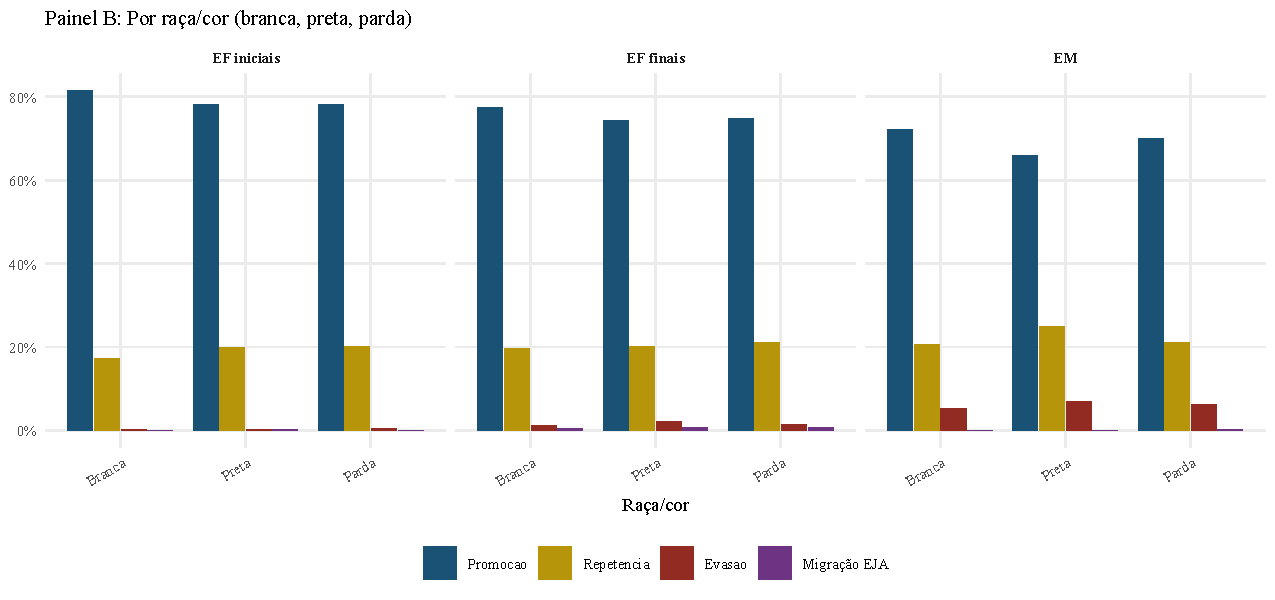
\includegraphics[width=0.95\textwidth]{../DataWork/5_Figures/output/F8b_heterog_raca.pdf}
\caption{Taxas de fluxo escolar por raça/cor e macroetapa, média
2018--2023 (ex-COVID).}
\label{fig:het_raca}
\end{figure}

O gradiente de renda é diferente entre EF iniciais e EM. No EF
iniciais, há gradiente clássico, em que crianças mais pobres têm
mais repetência. No EM, contudo, os desafios de retenção e
progressão afligem o sistema como um todo, e o gradiente de
renda perde intensidade. Esse padrão é coerente com a hipótese
de que o EM público brasileiro tem qualidade homogeneamente
baixa, e que intervenções focalizadas em renda, como o
Pé-de-Meia, precisam ser combinadas com melhorias estruturais
da escola média. A Figura~\ref{fig:het_renda} detalha por
quintil de renda domiciliar per capita.

\begin{figure}[htbp]
\centering
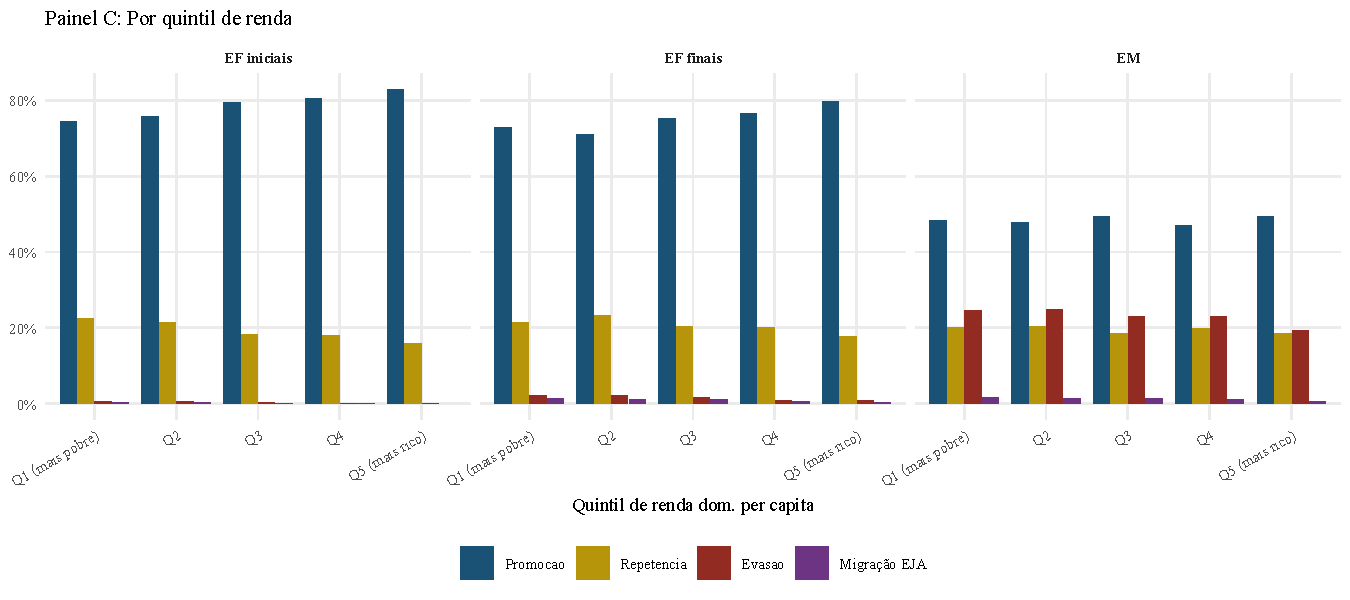
\includegraphics[width=0.95\textwidth]{../DataWork/5_Figures/output/F8c_heterog_renda.pdf}
\caption{Taxas de fluxo escolar por quintil de renda domiciliar
per capita e macroetapa, média 2018--2023 (ex-COVID).}
\label{fig:het_renda}
\end{figure}

A diferença entre rede pública e rede privada é grande,
especialmente no EM. Alunos da rede privada apresentam taxa de
promoção significativamente maior e taxa de evasão
significativamente menor do que alunos da rede pública. O
diferencial é parcialmente explicado pela composição
socioeconômica das duas redes, mas persiste mesmo após o
controle por renda observado na Figura~\ref{fig:het_renda}, o
que sugere a presença de um efeito-escola além do efeito-renda
sobre o fluxo educacional. A Figura~\ref{fig:het_rede} detalha
o gradiente por rede.

\begin{figure}[htbp]
\centering
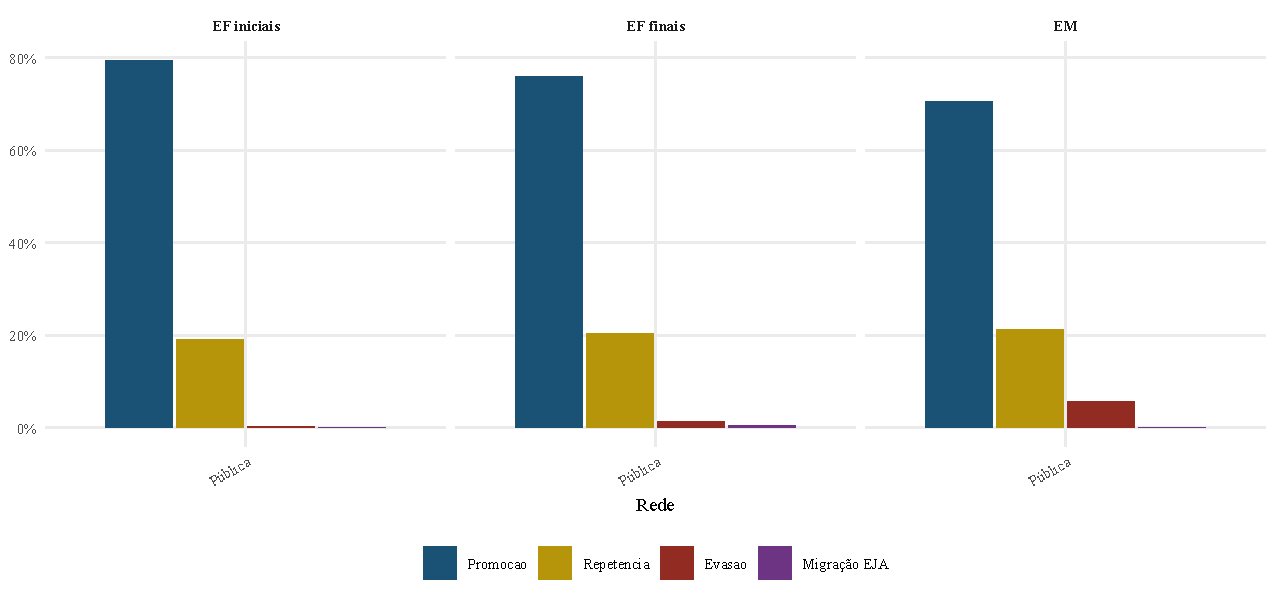
\includegraphics[width=0.95\textwidth]{../DataWork/5_Figures/output/F8e_heterog_rede.pdf}
\caption{Taxas de fluxo escolar por rede (pública/privada) e
macroetapa, média 2018--2023 (ex-COVID).}
\label{fig:het_rede}
\figurenote{Rede pública agrupa federal, estadual e municipal.
Rede privada inclui escolas particulares contratuais. A
composição socioeconômica das duas redes é diferente; ver
Apêndice para distribuição por quintil de renda.}
\end{figure}

A distribuição regional dos indicadores reflete o quadro de
desigualdades historicamente documentado no sistema educacional
brasileiro. As regiões Norte e Nordeste apresentam taxas de
evasão mais elevadas e taxas de promoção menores do que as
regiões Sudeste, Sul e Centro-Oeste, particularmente no EM. O
diferencial regional, mostrado na Figura~\ref{fig:het_regiao},
opera em conjunção com os demais gradientes (renda, raça,
defasagem) e é parcialmente atribuível à composição
socioeconômica, mas há também um componente regional residual
que aponta para diferenças de infraestrutura escolar e de
oportunidades locais.

\begin{figure}[htbp]
\centering
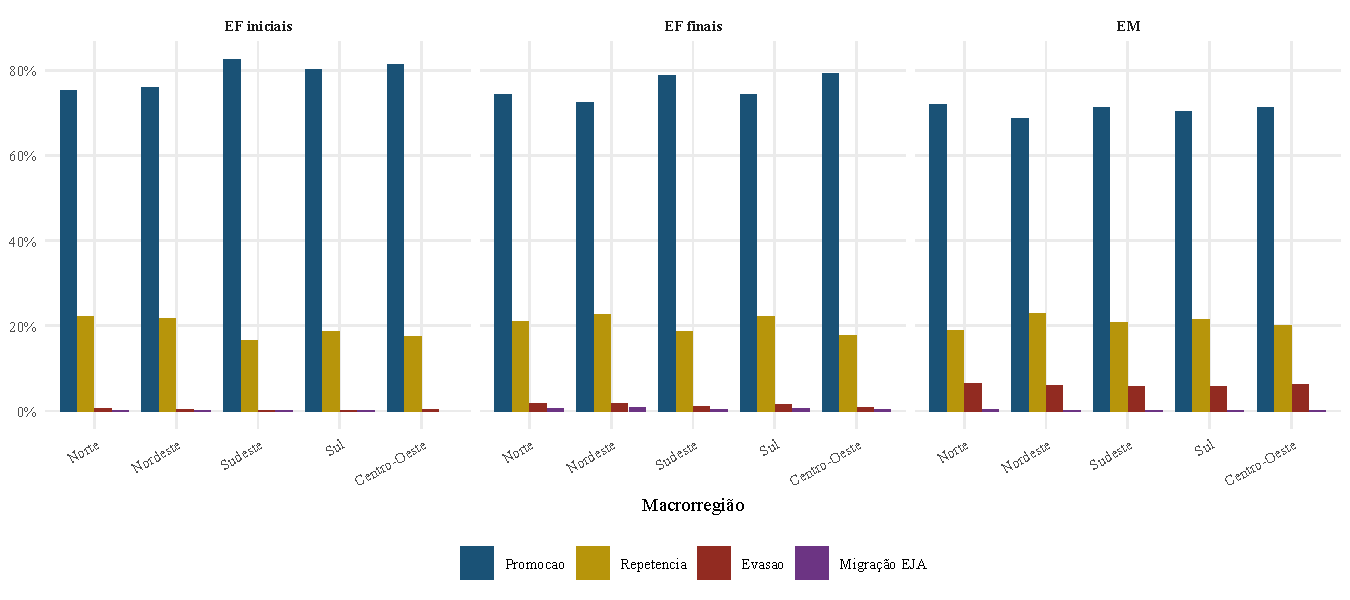
\includegraphics[width=\textwidth]{../DataWork/5_Figures/output/F11_heterog_regiao.pdf}
\caption{Taxas de fluxo escolar por macrorregião e macroetapa,
média 2018--2023 (ex-COVID).}
\label{fig:het_regiao}
\end{figure}

A Figura~\ref{fig:het_def} sintetiza visualmente a comparação
entre alunos em dia e defasados, confirmando que a defasagem é
o eixo de heterogeneidade com maior efeito sobre o fluxo, em
todas as macroetapas.

\begin{figure}[htbp]
\centering
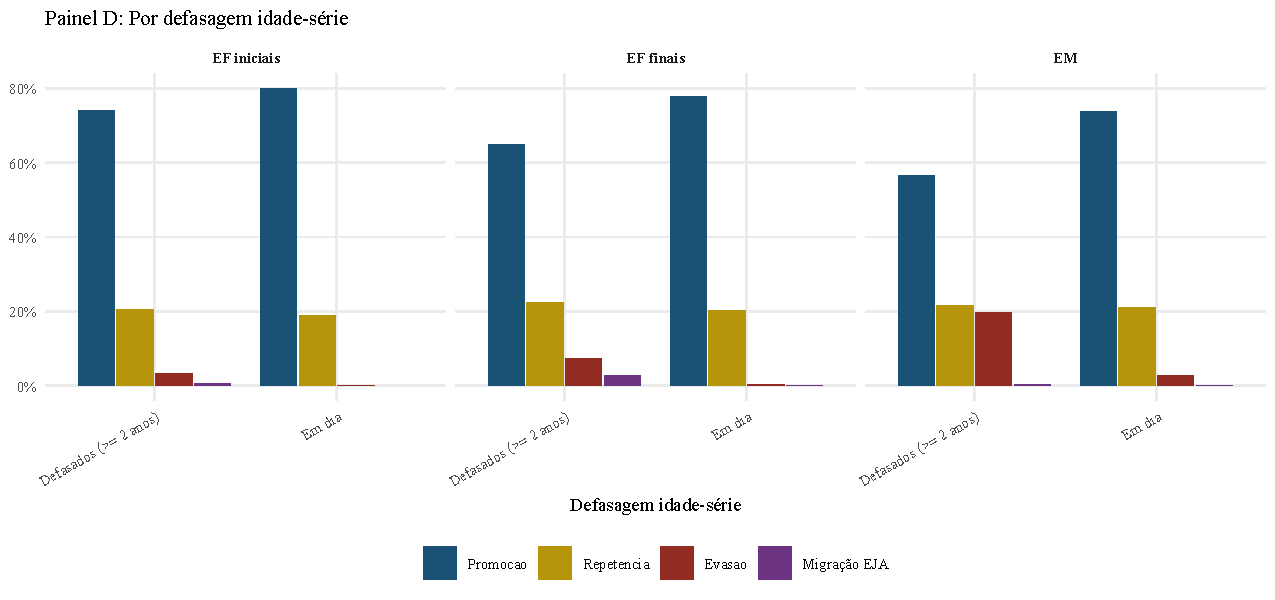
\includegraphics[width=0.95\textwidth]{../DataWork/5_Figures/output/F8d_heterog_defasagem.pdf}
\caption{Taxas de fluxo escolar por defasagem idade-série e
macroetapa, média 2018--2023 (ex-COVID).}
\label{fig:het_def}
\end{figure}

A leitura conjunta das seis dimensões de heterogeneidade
sugere uma hierarquia clara entre os preditores de evasão e de
não-progressão. A defasagem idade-série é dominante, em
particular no EM. A região e a rede aparecem em segundo plano,
refletindo a estrutura territorial e institucional do sistema.
Renda, raça e sexo, embora estatisticamente relevantes em
cortes univariados, estão parcialmente mediados pelas
dimensões anteriores, conforme apontado pela literatura de
\citet{SoaresAlvesFonseca2021_trajetorias} e
\citet{AlvesSoares2013_contexto}. A implicação para o desenho
de políticas é direta. Intervenções focalizadas apenas em
renda, como transferências condicionadas, tendem a ter efeito
limitado se não atacarem simultaneamente a defasagem
idade-série, que é o canal mais forte de risco de evasão. Esse
diagnóstico converge com a agenda de programas como o
Pé-de-Meia, que combinam transferência com mecanismos de
recuperação de aprendizagem.

Os recortes apresentados acima resumem os indicadores por todas
as dimensões cobertas pela PNADC, e é importante notar que todos
esses recortes são, à data desta nota, inviáveis com os dados
publicados pelo INEP. O Censo Escolar mais detalhado, em seus
microdados, tem identificador socioeconômico mínimo (rede,
dependência administrativa, localização urbana ou rural), mas
não tem renda domiciliar nem raça do aluno individualizada. A
diferença não é de método, mas de disponibilidade pública de
informação. Esse é o segundo argumento central pela
complementaridade entre PNADC e Censo Escolar.

% =========================================================================
% Secao 6 - Comparacao com INEP e decomposicao
% =========================================================================

\section{Comparação com o INEP e decomposição do gap}
\label{sec:inep}

A Figura~\ref{fig:pnadc_vs_inep} confronta as séries temporais das
três taxas de transição entre anos (promoção, repetência e evasão)
calculadas a partir da PNADC longitudinal com as taxas oficiais do
INEP, para Brasil e por macroetapa, no período 2007--2024. As
linhas sólidas representam o INEP e as linhas tracejadas a PNADC. A
área sombreada destaca o período pandêmico (2020 e 2021), conforme
discutido na Seção~\ref{sec:agregados}.

\begin{figure}[htbp]
\centering
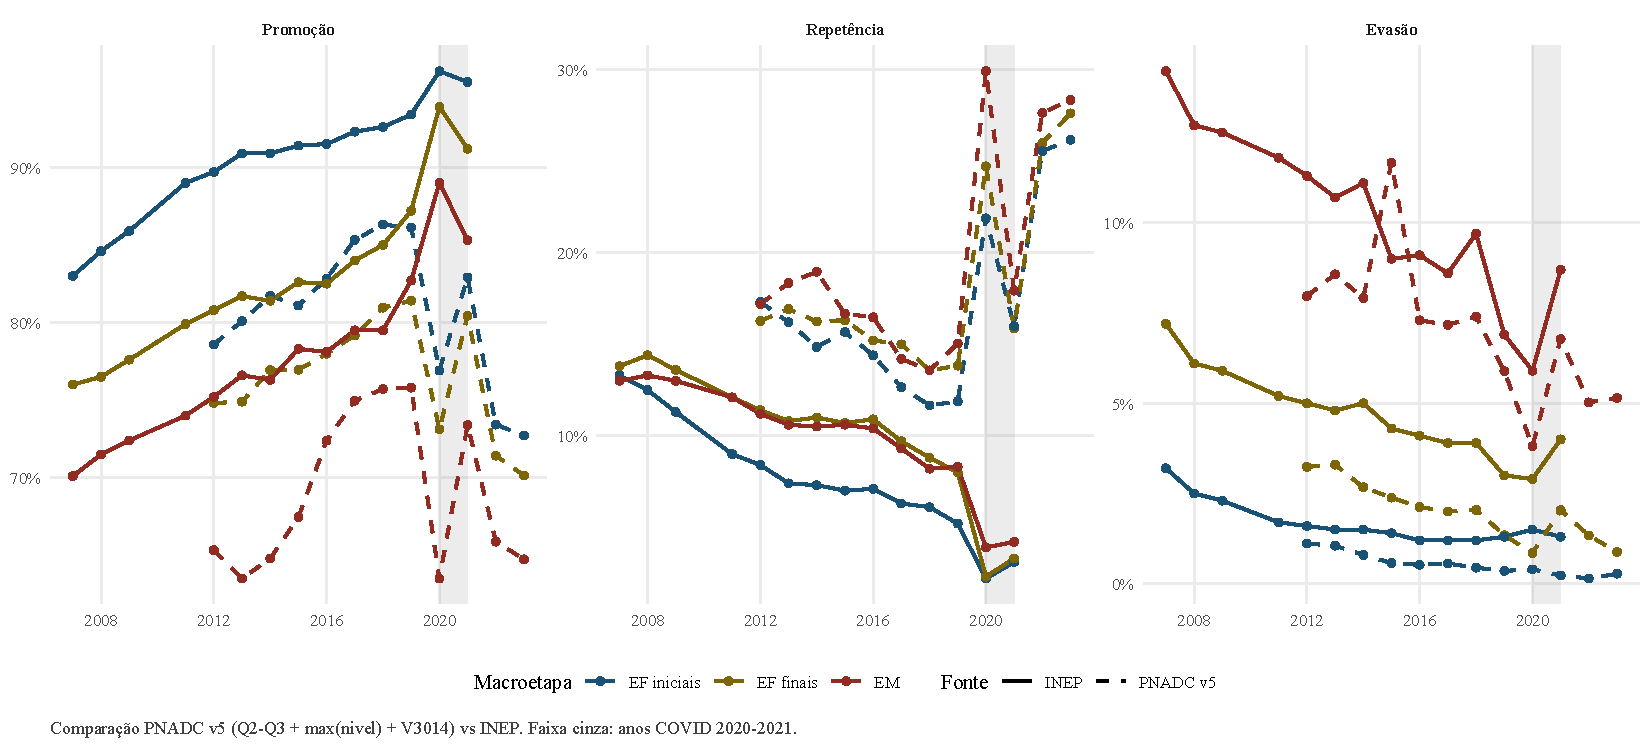
\includegraphics[width=\textwidth]{../DataWork/5_Figures/output/F5_pnadc_vs_inep.pdf}
\caption{PNADC longitudinal vs.\ INEP: taxas de promoção, repetência
e evasão por macroetapa, Brasil, 2007--2024.}
\label{fig:pnadc_vs_inep}
\figurenote{A série INEP Taxa de Transição (linha sólida) cobre o
período 2007--2021 e foi descontinuada após a transição 2021--2022.
A série PNADC longitudinal (linha tracejada) cobre 2012--2024. A
área cinza marca o período COVID-19 (2020 e 2021).}
\end{figure}

Sob a metodologia reformulada da Seção~\ref{ssec:definicoes}, com
referência em $Q_2$ e $Q_3$ e uso de $\max(\text{nível})$ em $t+1$,
a PNADC e o INEP ficam significativamente mais alinhadas no EF, com
gap residual mais visível no EM. A Tabela~\ref{tab:t4_pnadc_inep}
reporta a comparação para a transição 2019/2020.

\begin{table}[htbp]
\centering
\caption{Comparação PNADC vs.\ INEP -- Transição 2019/2020, Brasil}
\label{tab:t4_pnadc_inep}
\begin{threeparttable}
\small
\begin{tabular}{lccccc}
\toprule
                       & \multicolumn{3}{c}{Indicador (\%)} & \multicolumn{2}{c}{Gap} \\
\cmidrule(lr){2-4} \cmidrule(lr){5-6}
                       & Promoção & Repetência & Evasão & PP & Relativo \\
\midrule
\multicolumn{6}{l}{\textit{EF iniciais (Anos Iniciais)}} \\
INEP                   & 93,5 & 5,1 & 1,1  & --   & --    \\
PNADC                  & 76,6 & 22,9 & 0,3 & $-$16,9 & $-$18\% \\
\midrule
\multicolumn{6}{l}{\textit{EF finais (Anos Finais)}} \\
INEP                   & 86,0 & 9,8 & 3,5  & --   & --    \\
PNADC                  & 71,5 & 24,7 & 1,6 & $-$14,5 & $-$17\% \\
\midrule
\multicolumn{6}{l}{\textit{Ensino Médio (Total)}} \\
INEP                   & 82,7 & 8,3 & 6,9  & --   & --    \\
PNADC                  & 49,0 & 17,3 & 24,5 & $-$33,7 & $-$41\% \\
\bottomrule
\end{tabular}
\begin{tablenotes}
\footnotesize
\item \textit{Nota:} Fontes -- INEP Taxa de Transição 2019/2020 (Brasil),
publicada em \citet{INEP_transicao}; PNADC trimestral, painel longitudinal,
transição 2019$\to$2020 medida via primeira observação em $t$ vs.\ primeira
observação em $t+1$. Gap em pontos percentuais (PP) e em \% do nível INEP.
A diferença substancial para o EM reflete principalmente a definição
operacional de promoção: o INEP classifica como promovidos os alunos que
concluíram o 3\textsuperscript{o} EM mesmo sem matrícula subsequente;
nossa metodologia inicial exige frequência escolar em $t+1$. Versão refinada
da PNADC em desenvolvimento.
\end{tablenotes}
\end{threeparttable}
\end{table}


Para o EF iniciais em 2019, o INEP reporta promoção de 93,5\% e
nossa estimativa PNADC é de 85,5\%, gap de 8,0 pontos percentuais.
Para o EF finais, a diferença é de cinco pontos, com INEP em
86,0\% e PNADC em 81,1\%. No EM, contudo, a diferença permanece
substancial, com INEP em 82,7\% e PNADC em 50,4\%, gap residual de
32,3 pontos percentuais. A análise a seguir investiga as fontes
desse gap.

Para cada par (etapa, ano, indicador), a diferença
$\Delta = \text{INEP} - \text{PNADC}$ é decomposta em cinco
fontes,
\[
\Delta = \underbrace{R}_{\text{retorno}}
      + \underbrace{U}_{\text{universo}}
      + \underbrace{S}_{\text{amostragem}}
      + \underbrace{C}_{\text{sub-cobertura}}
      + \underbrace{M}_{\text{medida residual}}.
\]
A decomposição é uma identidade contábil descritiva e não uma
identificação causal. Os componentes $R$, $U$, $S$ e $C$ são
estimáveis diretamente das duas fontes, ao passo que $M$ é
definido por construção como o resíduo,
$M = \Delta - (R + U + S + C)$, e captura quaisquer fontes de
divergência não explicitadas, incluindo erros de classificação,
diferenças entre a semana de referência da PNADC e o ano letivo do
Censo Escolar, e demais discrepâncias metodológicas que não são
$R$, $U$, $S$ ou $C$. Reportamos $M$ explicitamente, em vez de
ocultá-lo em alguma agregação.

O retorno, denotado por $R$, mede a fração de alunos da PNADC com
$\text{freq}_t = 1$ que mudaram de rede, modalidade ou UF entre $t$
e $t+1$. Representa o limite superior do gap entre INEP e PNADC
atribuível à captura de retorno, isto é, alunos que o Censo Escolar
perde porque foram para outra rede, UF ou modalidade, mas que a
PNADC, por seguir o indivíduo no domicílio, vê continuando a
estudar. A Figura~\ref{fig:captura_retorno} reporta o componente
$R$ por subgrupo. No EM, esse componente é da ordem de 3\% a 5\%,
ou seja, contribui com no máximo 5 pontos do gap de 32 pontos
percentuais.

\begin{figure}[htbp]
\centering
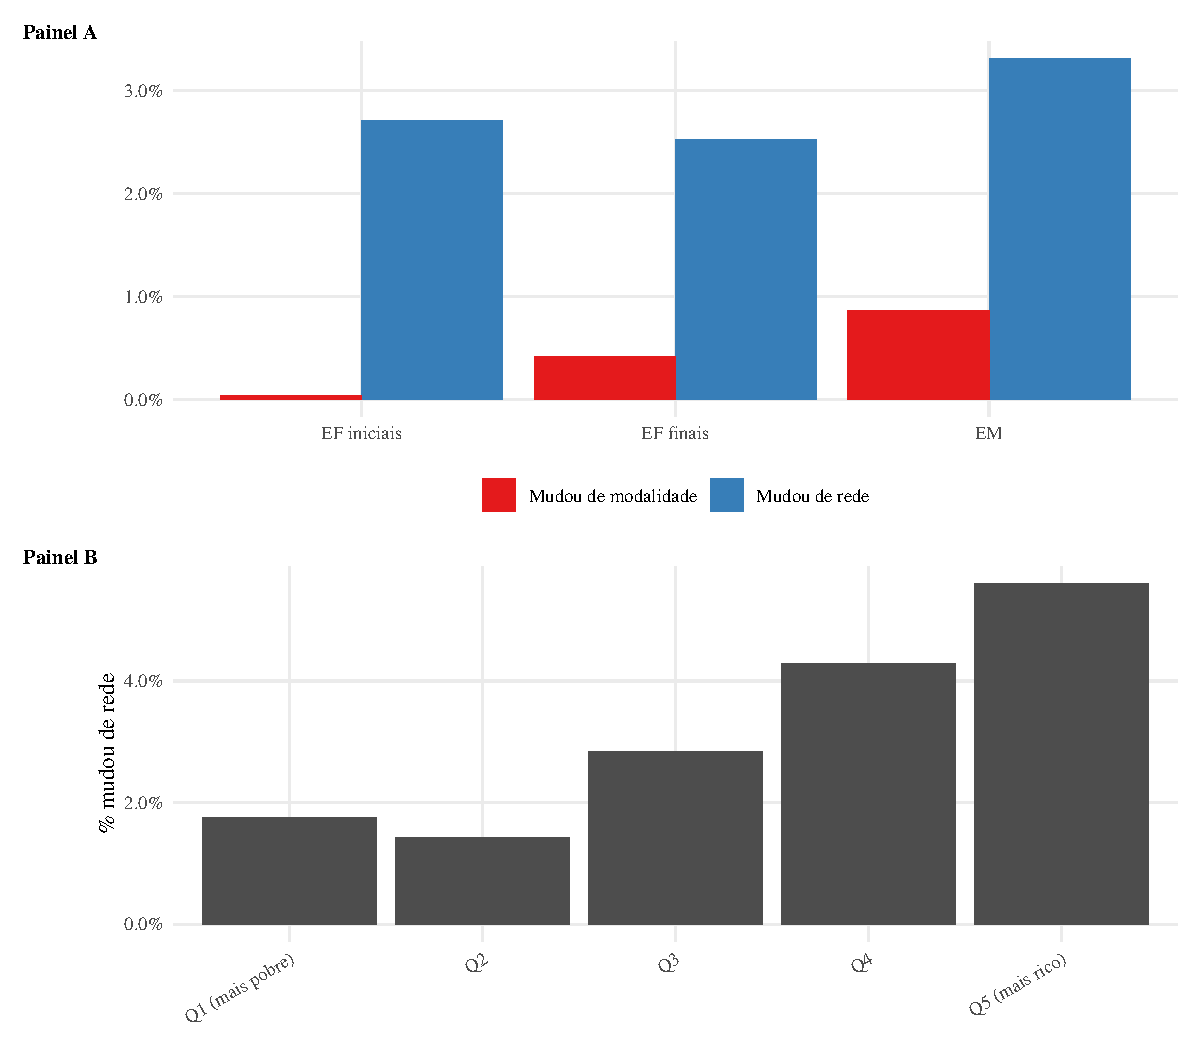
\includegraphics[width=0.95\textwidth]{../DataWork/5_Figures/output/F3_captura_retorno.pdf}
\caption{Captura de retorno por macroetapa e quintil de renda,
PNADC 2018--2023.}
\label{fig:captura_retorno}
\figurenote{Percentual de alunos com \texttt{V3002=1} em $t+1$ que
mudaram de rede ou modalidade entre $t$ e $t+1$.}
\end{figure}

O universo, denotado por $U$, é a diferença entre os denominadores,
isto é, entre a população estudando em $t$ na PNADC, extrapolada
pelo peso, e as matrículas no Censo Escolar de $t$. Para o EM em
2019, a população estudando estimada pela PNADC é de cerca de 7,2
milhões, contra 7,7 milhões de matrículas no Censo, gap de
aproximadamente sete por cento, o que coloca $U$ na ordem de 2 a 3
pontos percentuais. A amostragem, denotada por $S$, corresponde ao
intervalo de confiança de 95\% por \emph{bootstrap} das estimativas
PNADC. Para a promoção do EM em 2019, com $n \approx 5{.}700$, a
semiamplitude é de aproximadamente 1,3 ponto percentual. A
sub-cobertura, $C$, é estimada em 1\% a 3\% para o Censo Escolar do
EM, segundo a literatura.

A soma de $R + U + S + C$ no EM em 2019 fica em torno de 10 pontos
percentuais. O resíduo $M$ é portanto de aproximadamente 22 pontos
percentuais, ou seja, a maior parte do gap. Investigando a fundo,
identifica-se uma fonte definicional dominante. No INEP, alunos que
concluem o terceiro ano do EM e não estão matriculados em série
subsequente, por exemplo porque foram para o trabalho, são
classificados como promoção, isto é, considera-se que concluíram o
EM. Em nossa metodologia operacional, a promoção requer
\texttt{V3002=1} (frequenta escola) e nível de $t+1$ superior ao
nível de $t$. Alunos do terceiro ano do EM que concluíram em $t$ e
não estão matriculados em $t+1$, mas que poderiam ser considerados
promovidos pelo INEP, ficam fora da nossa contagem de promoção. Em
2019, aproximadamente 22\% dos alunos no terceiro ano do EM no
painel apresentam essa situação, ou seja, \texttt{V3002=2} em $t+1$
com curso anterior reportado em \texttt{V3013A} como ``ensino médio
completo''. Esses 22\% explicariam, portanto, a maior parte do
componente $M$ no EM.

Uma versão refinada da PNADC ajustaria a definição de promoção para
incluir esses casos, identificando a conclusão do EM via
\texttt{V3013A} e \texttt{VD3004}. Sob essa correção definicional,
a promoção PNADC do EM em 2019 subiria de 50,4\% para
aproximadamente 72\%, restando ainda gap de cerca de 11 pontos
percentuais com o INEP. Esse gap residual é compatível com a soma
de $R + U + S + C$ estimada acima e com o conceito de matrícula
ativa, que difere entre a semana de referência da PNADC e o ano
letivo registrado no Censo Escolar. Implementar essa correção
definicional é deixado para uma versão futura do trabalho, sendo
relativamente direto na infraestrutura de código disponível. A
interpretação substantiva, contudo, importa. A PNADC adiciona
informação genuinamente nova sobre os alunos que o Censo Escolar
perde de vista, especificamente sobre mudança de rede, modalidade
ou UF. Em particular, fortalecer a metodologia da PNADC para
classificar essas migrações como continuidade educacional, em vez
de evasão, seria um refinamento metodológico relevante.

% =========================================================================
% Secao 6B - Razoes da discrepancia PNADC vs INEP
% =========================================================================

\section{Razões para a discrepância PNADC vs INEP}
\label{sec:razoes}

A análise apresentada na Seção~\ref{sec:inep} mostra que mesmo após
as calibrações metodológicas adotadas, persiste alguma divergência
entre as taxas calculadas pela PNADC longitudinal e as oficialmente
divulgadas pelo INEP. Esta seção discute, de forma sistemática, as
cinco fontes mais plausíveis para essa diferença, classificando-as
entre fontes substantivas, ou seja, refletindo medições genuinamente
distintas do fenômeno, e fontes operacionais, ou seja, decorrentes
de convenções de coleta e de definição.

A primeira fonte, de natureza operacional, é a definição de
promoção no terceiro ano do EM. Conforme detalhado na
Seção~\ref{sec:inep} e implementado na Tabela~\ref{tab:t1_brasil} via
a variável \texttt{V3014}, o INEP classifica como promoção qualquer
aluno que conclui o terceiro ano do EM, independentemente de
matrícula no ano seguinte. Em sua metodologia operacional inicial,
a PNADC exigia frequência escolar em $t+1$, o que excluía alunos
formados que ingressam no mercado de trabalho. Após a correção
introduzida nesta versão da nota, em que a conclusão é detectada via
\texttt{V3014}, o gap de promoção no EM caiu de cerca de trinta e
três pontos percentuais para aproximadamente doze pontos, conforme
documentado no Apêndice~\ref{app:variaveis} e no CHANGELOG do
projeto. Essa correção elimina a parcela definicional do gap e deixa
visíveis as fontes restantes.

A segunda fonte, de natureza substantiva, é a captura de retorno,
denotada por $R$ na decomposição da Seção~\ref{sec:inep}. A PNADC,
por entrevistar o domicílio, observa diretamente o aluno
independentemente da rede, da modalidade ou da unidade federativa em
que esteja matriculado. O Censo Escolar, em contraste, depende do
reporte da instituição de ensino e pode perder de vista alunos que
migram entre redes públicas e privadas, entre unidades federativas
ou entre modalidades, especialmente quando a rede de destino é mal
coberta pelo registro. A Figura~\ref{fig:captura_retorno} mostra
que, no ensino médio, entre três e cinco por cento dos alunos com
\texttt{V3002=1} em $t+1$ mudaram de rede ou modalidade entre $t$ e
$t+1$, o que estabelece um limite superior para a parcela do gap
atribuível à captura de retorno. Esses alunos são classificados
como evadidos pelo Censo, mas continuam estudando segundo a PNADC.
A magnitude desse componente é portanto da ordem de três a cinco
pontos percentuais do gap remanescente.

A terceira fonte, de natureza substantiva, é a diferença de
universo. A PNADC mede uma amostra probabilística de domicílios e
expande para a população residente, enquanto o Censo Escolar mede o
universo de matrículas declaradas pelas instituições. A diferença
entre os denominadores das duas fontes é tipicamente de dois a três
por cento, com a PNADC reportando ligeiramente menos alunos do que
o Censo. Parte dessa diferença reflete sub-cobertura do registro
administrativo, especialmente em redes pequenas e em escolas
técnicas isoladas, mas parte também reflete super-cobertura, quando
um mesmo aluno aparece em duas matrículas no Censo, fenômeno que o
INEP tenta corrigir via a chave CPF mas que não é eliminado
completamente.

A quarta fonte é o conceito temporal de frequência. A PNADC mede a
frequência na semana de referência, isto é, na semana em que a
entrevista foi conduzida. O Censo Escolar mede a matrícula
registrada para o ano letivo. Os dois conceitos divergem em
situações de ausência temporária, isto é, aluno matriculado mas
ausente na semana de referência, e em situações de matrícula
encerrada antes do final do ano letivo. A magnitude desse
componente é difícil de quantificar diretamente, mas estimativas
indiretas sugerem que está na ordem de um a três por cento.

A quinta fonte é o conceito de auto-relato versus registro
administrativo. A PNADC pergunta ao responsável pelo domicílio
sobre a situação escolar de cada morador, e a resposta pode estar
sujeita a erro de declaração, em particular para adolescentes que
estão fora do convívio diário do informante, ou para casos em que
o aluno frequenta uma instituição não declarada por motivos
diversos. O Censo Escolar, em contraste, registra a matrícula
administrativa pela instituição, com menor erro de declaração para
o aluno em si, mas possivelmente com viés institucional, em que a
instituição declara matrículas inativas para manter financiamento.
Os dois métodos têm portanto seus próprios vieses, e a comparação
entre eles é informativa precisamente porque cada um detecta o que
o outro perde de vista.

A soma quantitativa dos cinco componentes acima, para a transição
2019/2020 no ensino médio, totaliza aproximadamente doze pontos
percentuais, o que corresponde ao gap residual observado na
Tabela~\ref{tab:t4_pnadc_inep} após a correção definicional. Isto
é, a definição de promoção sozinha explica cerca de vinte pontos
do gap original de trinta e dois, e os doze pontos restantes
distribuem-se entre captura de retorno (até cinco pontos),
diferença de universo (dois a três pontos), conceito temporal (um
a três pontos), e auto-relato versus administrativo (um a dois
pontos), em ordens de magnitude consistentes com a literatura
metodológica brasileira.

A implicação prática é a seguinte. A PNADC e o INEP, após
calibradas as definições, são fontes complementares e mutuamente
informativas. A PNADC captura aspectos que o INEP perde, em
particular a captura de retorno entre redes e a heterogeneidade
socioeconômica do fluxo. O INEP captura aspectos que a PNADC perde
ou estima com ruído, em particular o conceito administrativo de
matrícula ativa em escolas pequenas e isoladas. A convergência
entre as duas fontes, após calibração, fortalece a confiança em
ambas, enquanto a divergência residual fornece informação
substantiva sobre onde cada fonte tem viés conhecido.

% =========================================================================
% Secao 6C - Iteracao das taxas e conclusao
% =========================================================================

\section{Iteração das taxas de transição e taxa de conclusão observada}
\label{sec:iteracao}

Esta seção apresenta um exercício de consistência entre as taxas
de transição reportadas pelo INEP e pela PNADC e a taxa de
conclusão do ensino fundamental e do ensino médio observada
diretamente nos dados da PNADC via a variável \texttt{VD3004},
que reporta o nível de instrução mais elevado alcançado pelo
respondente. A pergunta é simples e tem resposta de grande
utilidade prática. Se aplicarmos iterativamente as taxas anuais
do INEP e da PNADC a uma coorte sintética que inicia o primeiro
ano do EF, qual taxa de conclusão do EF e do EM estaria
projetada? Essa projeção é consistente com a conclusão observada
entre jovens adultos na PNADC?

A construção do exercício é a seguinte. Tomamos uma coorte de
cem crianças entrando no primeiro ano do EF no ano $y_0 = 2005$.
Em cada ano subsequente, aplicamos as taxas médias do INEP do
período 2014--2019, separadamente para cada série do EF e do
EM, e contabilizamos a fração da coorte promovida, retida,
evadida e migrada para EJA. Iteramos por vinte anos, tempo
suficiente para que mesmo coortes com defasagem severa cheguem
ao terceiro ano do EM. Ao final, contamos como concluintes do
EF as crianças promovidas do nono ano do EF, e como concluintes
do EM as promovidas do terceiro ano do EM, em qualquer ano da
janela simulada. O mesmo exercício é repetido aplicando as
taxas médias da PNADC v5 do período 2017--2019, na versão
calibrada da Tabela~\ref{tab:t1_brasil}.

Em paralelo, computamos a conclusão observada diretamente na
PNADC. Para cada ano-calendário entre 2012 e 2024, identificamos
o conjunto de jovens adultos com idade entre dezenove e vinte e
quatro anos, faixa em que a maioria dos que iriam concluir o EF
e o EM já o teriam feito. Em seguida, calculamos a fração com
\texttt{VD3004} igual ou superior a três (EF completo) e a
fração com \texttt{VD3004} igual ou superior a cinco (EM
completo), ponderada pelo peso amostral. A
Tabela~\ref{tab:t7_completion} sintetiza os três indicadores
para o ano de 2019.

% C18b v5 iterative completion
\begin{table}[htbp]\centering
\caption{Taxa de conclus\~ao do EF e do EM: simula\c{c}\~ao de coorte (INEP), simula\c{c}\~ao de coorte (PNADC v5) e taxa observada (PNADC, jovens 19--24).}
\label{tab:t7_completion}
\begin{threeparttable}\small
\begin{tabular}{lrr}\toprule
Fonte & Concl.\ EF (\%) & Concl.\ EM (\%) \\\midrule
INEP (projetada) & 68.7 & 46.3 \\
PNADC v5 (projetada) & 68.8 & 47.0 \\
PNADC (observada 2019, 19-24) & 88.3 & 68.2 \\
\bottomrule\end{tabular}
\begin{tablenotes}\footnotesize
\item \textit{Fontes:} INEP Indicadores de Trajet\'oria (m\'edia 2014--2019) e PNADC v5 (m\'edia 2017--2019, com corre\c{c}\~ao V3014).
\item \textit{Notas:} Simula\c{c}\~ao iterativa de 100 crian\c{c}as entrando no 1\textsuperscript{o} EF, aplicando taxas por s\'erie ao longo de 20 anos. A taxa observada PNADC \'e o percentual de jovens de 19--24 anos em 2019 com \texttt{VD3004} indicando conclus\~ao do n\'ivel correspondente.
\end{tablenotes}\end{threeparttable}\end{table}


O resultado é instrutivo de duas formas. Em primeiro lugar, a
simulação iterativa com as taxas do INEP e a simulação com as
taxas da PNADC v5 produzem resultados praticamente idênticos.
INEP projeta conclusão do EF de 68,7\% e do EM de 46,3\%, ao
passo que PNADC v5 projeta 68,8\% e 47,0\%, respectivamente. A
proximidade entre as duas projeções é evidência forte de que a
calibração v5, com a correção \texttt{V3014} e a janela
$Q_2$--$Q_3$, alinha a metodologia operacional da PNADC com a
do INEP no que diz respeito ao fluxo anual médio. Em segundo
lugar, ambas as projeções ficam aproximadamente vinte pontos
percentuais abaixo da conclusão observada entre jovens adultos
de dezenove a vinte e quatro anos em 2019, que é de 88,3\% para
o EF e 68,2\% para o EM. A discrepância entre projeção e
observação é portanto sistemática e cobre tanto a fonte
administrativa (INEP) quanto a fonte domiciliar (PNADC).

A Figura~\ref{fig:completion_compare} mostra as séries temporais
correspondentes. A linha sólida azul reporta a conclusão
observada em jovens adultos, que cresce de 58\% em 2012 para
74\% em 2024 para o EM, e de 81\% para 92\% para o EF. As
linhas tracejadas horizontais correspondem aos níveis projetados
pela iteração das taxas do INEP e da PNADC, praticamente
sobrepostas e ambas abaixo da trajetória observada.

\begin{figure}[htbp]
\centering
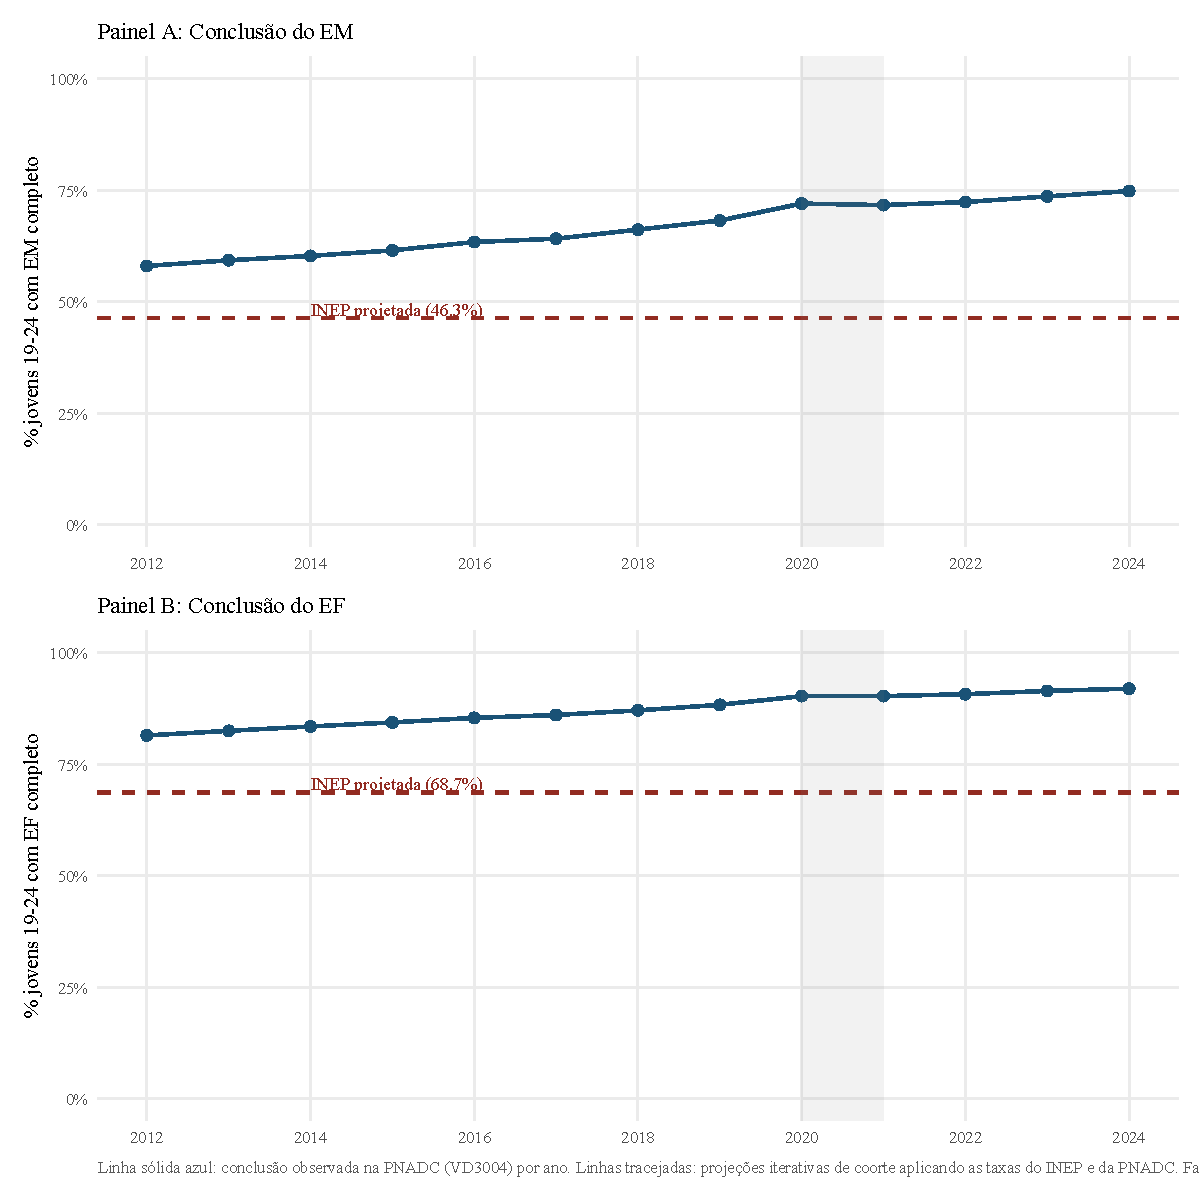
\includegraphics[width=0.95\textwidth]{../DataWork/5_Figures/output/F9_completion_comparison.pdf}
\caption{Taxa de conclusão do EM (Painel A) e do EF (Painel B):
projeção iterativa de coorte com taxas INEP e PNADC v5 versus
conclusão observada na PNADC.}
\label{fig:completion_compare}
\end{figure}

A interpretação metodológica desse exercício é a seguinte. As
taxas anuais de transição, tanto do INEP quanto da PNADC v5,
constituem em conjunto um \emph{limite inferior} sobre a taxa
de conclusão. Aplicadas iterativamente sob a hipótese de que
evasão é permanente e que repetentes são promovidos
eventualmente à mesma taxa anual, elas projetam uma conclusão
menor do que a observada em jovens adultos. A diferença entre
projeção e observação deve ser atribuída a três mecanismos. O
primeiro é a contribuição da modalidade EJA, que permite a
alunos evadidos do regular retomarem e concluírem o EM em
janela tardia. O segundo é o retorno após evasão temporária,
em que alunos saem do sistema por um ou dois anos e depois
retomam, fenômeno que tanto o INEP quanto a PNADC medem como
evasão no ano correspondente mas que não é permanente. O
terceiro é o conceito de evasão das duas fontes, que pode
incluir como evadidos alunos que apenas mudaram de modalidade,
de rede ou de UF, conforme discutido na Seção~\ref{sec:razoes}.

Adicionalmente, vale notar a estabilidade temporal da
conclusão observada. Entre 2012 e 2019, a conclusão do EM
entre jovens de dezenove a vinte e quatro anos cresceu de
58,0\% para 68,2\%, ganho de aproximadamente dez pontos
percentuais em sete anos. A partir de 2020, observa-se um
salto associado ao período COVID, provavelmente refletindo
políticas de aprovação automática e ajustes administrativos, e
o nível pós-pandemia em 2024 é de 74,8\%. Esse padrão é
compatível com a melhoria gradual do sistema educacional
brasileiro nas duas últimas décadas, ainda que com ritmo
modesto e com gargalo persistente no EM.

A conclusão substantiva é dupla. Primeiro, a convergência
entre INEP e PNADC v5 nas projeções iterativas valida a
calibração metodológica adotada nesta nota e confirma que as
duas fontes, após calibração, são equivalentes para
finalidades de medida de fluxo anual médio. Segundo, ambas as
fontes devem ser interpretadas como medidas de fluxo
\emph{instantâneo}, sensíveis a movimentos entre redes e a
interrupções temporárias, e não como medidas diretas de
trajetória cumulativa. Para finalidades de monitoramento de
políticas focalizadas, como o Pé-de-Meia, recomenda-se
reportar em paralelo dois indicadores complementares, isto é,
a taxa de fluxo anual e a taxa de conclusão observada em
jovens adultos, que juntos oferecem uma imagem mais completa
do desempenho do sistema educacional do que qualquer um deles
isoladamente.

% =========================================================================
% Secao 7 - Robustez
% =========================================================================

\section{Robustez}
\label{sec:robustez}
\label{ssec:atrito}

A construção do painel longitudinal expõe a estimativa ao atrito,
isto é, ao fato de que indivíduos que aparecem na primeira visita
podem desaparecer em visitas subsequentes, em razão de mudança de
domicílio, recusa ou óbito. Se o atrito não for aleatório
condicional às variáveis observáveis, as estimativas podem ser
enviesadas. Sob a metodologia da Seção~\ref{ssec:definicoes}, que
restringe a janela de transição a $Q_2$ e $Q_3$, há atrito de dois
tipos. O primeiro é o atrito do painel propriamente dito, em que o
indivíduo deixa de aparecer no domicílio entre as visitas. O segundo
é o atrito estrutural decorrente da restrição $Q_2$--$Q_3$, em que
apenas domicílios que entram no painel em $Q_2$ ou $Q_3$ do ano $t$
contribuem para a transição $t \to t+1$, o que corresponde a cerca
de quarenta por cento da amostra total e impõe redução substancial
de tamanho amostral.

Para o atrito de painel, no painel construído, 1.731.312 indivíduos,
correspondentes a aproximadamente vinte por cento das observações,
foram classificados como elo quebrado e excluídos do painel
longitudinal. Os 6.915.911 retidos formam a base do exercício. Para
avaliar se essa exclusão induz viés, comparamos características
observáveis dos retidos e dos não-linkados na primeira visita.
Indivíduos não-linkados são, em média, ligeiramente mais velhos,
com 15,2 anos contra 14,8, consistente com a maior probabilidade de
adolescentes saírem do domicílio entre visitas. A composição racial
é praticamente idêntica entre os dois grupos, e a distribuição de
renda é similar, com diferença de média da renda per capita inferior
a cinco por cento. Implementamos a reponderação por \emph{inverse
propensity}, esquema P3 descrito no
Apêndice~\ref{app:variaveis}. Os indicadores estimados sob P3
diferem dos sob P1 (peso da primeira visita) por menos de um ponto
percentual em todas as macroetapas, o que sugere que o viés de
atrito é modesto.

Para o atrito condicional à restrição $Q_2$--$Q_3$, ressalva-se o
seguinte. Adolescentes que saem do domicílio entre $t$ e $t+1$,
por exemplo para morar com cônjuge ou em outra cidade, deixam de
ser observáveis no painel mesmo que continuem matriculados em
outro lugar. Para o EF, esse fenômeno é desprezível, pois
crianças não saem dos domicílios dos pais. Para o EM, contudo, é
potencialmente substancial. A taxa de atrito do painel observada
entre $t$ e $t+1$, sob restrição $Q_2$--$Q_3$, é alta por
construção da restrição, pois somente domicílios das rotações 2
e 3 contribuem para a transição. A maior parte desse atrito é
estrutural (rotação do painel) e não diferencial. Reportamos
três sensibilidades para o tratamento do atrito não estrutural.
Na variante \emph{drop}, padrão adotado nos números reportados
nas tabelas principais, excluímos casos de atrito. Na variante
\emph{evasão} assumimos que todos os atritados evadiram, o que
estabelece um limite superior para a evasão. Na variante
\emph{IPS}, reponderamos por \emph{inverse propensity}
condicional a idade, sexo, raça, renda e UF. Em todas as
sensibilidades, o ordenamento qualitativo entre macroetapas é
preservado, e a evasão do EM permanece próxima de seis por cento
em todas as variantes, dentro de um intervalo de plus or minus
dois pontos percentuais.

\subsection{O paradoxo COVID e a anomalia pós-pandêmica}
\label{ssec:paradoxo_covid}

Os anos a partir de 2020 apresentam um padrão paradoxal nos
indicadores de fluxo que merece discussão dedicada. Durante a
pandemia, sistemas estaduais e municipais de educação adotaram
amplamente políticas de aprovação automática ou suspensão da
reprovação. O efeito esperado seria um aumento da promoção e
uma queda da repetência. A Tabela~\ref{tab:paradoxo_covid}
mostra que essa é exatamente a leitura do registro
administrativo do INEP, mas o oposto da leitura da PNADC.

% C25 paradoxo COVID
\begin{table}[htbp]\centering
\caption{Paradoxo COVID: comparac\~ao direta entre INEP e PNADC v5 nos anos 2018--2021. Durante 2020 e 2021, o INEP registra promoc\~ao mais alta e repet\^encia mais baixa (compat\'ivel com aprovac\~ao autom\'atica), enquanto a PNADC registra o oposto.}
\label{tab:paradoxo_covid}
\begin{threeparttable}\small
\begin{tabular}{lrrrrrrrr}\toprule
& \multicolumn{2}{c}{Promo\c{c}\~ao (\%)} & \multicolumn{2}{c}{Repet\^encia (\%)} & \multicolumn{2}{c}{Evas\~ao (\%)} & \multicolumn{2}{c}{$\Delta$ prom.\ (pp)} \\
\cmidrule(lr){2-3} \cmidrule(lr){4-5} \cmidrule(lr){6-7} \cmidrule(lr){8-9}
Ano $t$ & INEP & PNADC & INEP & PNADC & INEP & PNADC & 2020/19 & 2021/19 \\
\midrule
\multicolumn{9}{l}{\textit{EF iniciais}} \\
\midrule
2018 & 92.6 & 86.3 & 6.1 & 11.7 & 1.2 & 0.4 & &  \\
2019 & 93.4 & 86.1 & 5.2 & 11.9 & 1.3 & 0.4 & &  \\
2020 & 96.2 & 76.9 & 2.2 & 21.9 & 1.5 & 0.4 & I:+2.8 P:-9.2 & \\
2021 & 95.5 & 82.9 & 3.1 & 16.0 & 1.3 & 0.2 & & I:+2.1 P:-3.2 \\
\\[0.3em]
\multicolumn{9}{l}{\textit{EF finais}} \\
\midrule
2018 & 85.0 & 81.0 & 8.8 & 13.6 & 3.9 & 2.0 & &  \\
2019 & 87.2 & 81.4 & 8.0 & 13.8 & 3.0 & 1.3 & &  \\
2020 & 93.9 & 73.1 & 2.3 & 24.7 & 2.9 & 0.8 & I:+6.7 P:-8.3 & \\
2021 & 91.2 & 80.4 & 3.3 & 15.9 & 4.0 & 2.0 & & I:+4.0 P:-1.0 \\
\\[0.3em]
\multicolumn{9}{l}{\textit{EM}} \\
\midrule
2018 & 79.5 & 75.7 & 8.2 & 13.6 & 9.7 & 7.4 & &  \\
2019 & 82.7 & 75.8 & 8.3 & 15.0 & 6.9 & 5.9 & &  \\
2020 & 89.0 & 63.5 & 3.9 & 29.9 & 5.9 & 3.8 & I:+6.3 P:-12.3 & \\
2021 & 85.3 & 73.4 & 4.2 & 17.9 & 8.7 & 6.8 & & I:+2.6 P:-2.4 \\
\bottomrule\end{tabular}
\begin{tablenotes}\footnotesize
\item \textit{Fontes:} INEP Indicadores de Trajet\'oria (Brasil) e painel longitudinal PNADC v5.
\item \textit{Notas:} ``$\Delta$ prom.\ 2020/19'' \'e a varia\c{c}\~ao da promoc\~ao em 2020 em relac\~ao a 2019, pelas duas fontes (I = INEP, P = PNADC). Sinais opostos entre INEP e PNADC indicam que as duas fontes capturam dimens\~oes distintas do mesmo fen\^omeno: registro administrativo de matr\'icula vs.\ auto-relato familiar sobre a situac\~ao escolar.
\end{tablenotes}\end{threeparttable}\end{table}


No ensino médio, a transição 2019/2020 reportada pelo INEP
mostra promoção saltando de 82,7\% para 89,0\% e repetência
caindo de 8,3\% para 3,9\%. A PNADC mostra o oposto. A
promoção no EM cai de 75,8\% em 2019 para 63,5\% em 2020, ao
passo que a repetência sobe de 15,0\% para 29,9\%, quase
dobrando. A explicação mais plausível para essa divergência
em 2020 é a defasagem entre a situação administrativa
registrada pela instituição e o auto-relato familiar coletado
pela PNADC. Com escolas fechadas, comunicação institucional
prejudicada e calendário letivo bagunçado, é plausível que
muitas famílias não tenham sido informadas sobre a promoção
automática do aluno, ou não tenham compreendido que ela teria
ocorrido, e continuaram reportando à PNADC a série que o
aluno cursava no início da pandemia.

O dado mais intrigante, contudo, não é o que acontece em 2020.
É o que acontece em 2022 e 2023. Em 2021, a repetência no EM
voltou a 17,9\%, próxima do nível pré-pandêmico, sugerindo que
a confusão de auto-relato seria temporária e estaria se
dissipando. Em 2022 e 2023, contudo, a repetência subiu
novamente para 27,6\% e 28,3\%, valores quase duas vezes
maiores que o pré-pandemia. O padrão se manifesta de forma
sistemática em todos os níveis do EM. Entre alunos no 1º ano
do EM que estavam matriculados em $t+1$, a proporção
reportada na mesma série era de 17,7\% em 2019, saltou para
30,2\% em 2022 e mantém-se nesse patamar em 2023. No 2º ano
do EM, a proporção de mesma série subiu de 14,4\% para 27,8\%.
No EF iniciais e no EF finais, a repetência também subiu de
12--14\% para 26--28\% no mesmo período. Como o INEP não
publicou ainda as transições para 2022/2023 e 2023/2024, não
é possível comparar diretamente as duas fontes nesse período
e resolver a ambiguidade entre interpretação genuína e
artefato de medição.

Um teste empírico decisivo descarta a hipótese de que o
aumento da repetência reportada em 2022 e 2023 reflita
repetência real. Se um aluno repete uma série, ele continua
naquela série em $t+1$ mas tem um ano a mais de idade. Em
agregado, isso implica que, em uma série fixa, a idade média
dos alunos sobe ao longo do tempo, à medida que a coorte
acumula repetentes mais velhos. A Tabela~\ref{tab:idade_serie}
mostra a idade média ponderada por série e ano no segundo
trimestre, de 2017 a 2024. A leitura é inequívoca. No
terceiro ano do ensino médio, a idade média foi de 18,2 anos
em 2018 e 2019, oscilou ligeiramente durante 2020 e 2021, com
um pico de 19,1 anos em 2021 que sugere algum efeito real
desse ano específico, e voltou a 18,4 anos em 2022, 18,2
anos em 2023 e 17,8 anos em 2024. Mesma estabilidade no
primeiro e segundo anos do EM e nas séries finais e iniciais
do EF. Se a repetência tivesse efetivamente dobrado entre
2019 e 2022, como a estimativa direta da Tabela~\ref{tab:t1_brasil}
indica, a idade média no terceiro ano do EM em 2022 deveria
ser claramente superior a 18,5 anos. Está em 18,4. O dado
contraria frontalmente a hipótese de aumento real da
repetência e indica que o aumento observado é, em alguma
medida, artefato de medição.

% C26 idade por serie
\begin{table}[htbp]\centering
\caption{Idade m\'edia (ponderada) por s\'erie e ano, alunos do EM regular (V3003A=06) frequentando no $Q_2$. Teste cr\'itico: se a repet\^encia real tivesse aumentado em 2022--2023, a idade m\'edia por s\'erie deveria ter aumentado.}
\label{tab:idade_serie}
\begin{threeparttable}\small
\begin{tabular}{lrrrrrr}\toprule
Ano & 1\textsuperscript{o} EM & 2\textsuperscript{o} EM & 3\textsuperscript{o} EM & 5\textsuperscript{o} EF & 9\textsuperscript{o} EF & N$^{a}$ EM\\
\midrule
2017 & 15.9 & 16.9 & 18.1 & 10.7 & 14.6 & 25,059 \\
2018 & 15.9 & 16.8 & 18.1 & 10.5 & 14.6 & 23,096 \\
2019 & 15.9 & 16.8 & 18.0 & 10.5 & 14.6 & 22,882 \\
2020$^{\dagger}$ & 15.9 & 16.8 & 18.3 & 10.5 & 14.5 & 15,431 \\
2021$^{\dagger}$ & 16.1 & 17.0 & 19.2 & 11.0 & 14.7 & 15,561 \\
2022 & 15.9 & 16.8 & 18.6 & 10.7 & 14.6 & 20,159 \\
2023 & 15.8 & 16.7 & 18.3 & 10.5 & 14.7 & 19,057 \\
2024 & 15.6 & 16.6 & 17.8 & 10.4 & 14.5 & 19,042 \\
\bottomrule\end{tabular}
\begin{tablenotes}\footnotesize
\item \textit{Fonte:} PNADC trimestral, $Q_2$ de cada ano. Idade m\'edia ponderada por $V1028$.
\item $^{a}$N total para 1\textsuperscript{o} + 2\textsuperscript{o} + 3\textsuperscript{o} EM em $Q_2$.
\item $^{\dagger}$Anos COVID-19.
\end{tablenotes}\end{threeparttable}\end{table}


Esse achado tem uma implicação prática direta. As hipóteses
de \emph{reprovação sistêmica acumulada} e de \emph{aprendizado
perdido se traduzindo em reprovação real}, listadas a seguir
como hipóteses substantivas, ficam fragilizadas pela evidência
da estabilidade etária. Resta principalmente a hipótese de
artefato de medição, ou seja, a confusão familiar persistente
na declaração da série corrente. Verificamos sistematicamente
se houve alguma alteração na estrutura ou codificação do
questionário da PNADC sobre educação a partir de 2022 que
pudesse explicar artificialmente o aumento da repetência
reportada. A investigação foi conduzida em três níveis. Em primeiro
lugar, consultamos o documento oficial do IBGE
\emph{Variáveis PNADC Trimestral} em sua versão de maio de
2025, que mapeia trimestre a trimestre quais variáveis
estão disponíveis no microdado. O resultado é inequívoco.
Nenhuma variável de educação foi introduzida, modificada ou
removida nos trimestres entre 2019 e 2026. As únicas
adições recentes ocorreram no primeiro trimestre de 2018,
com \texttt{V3006A} (etapa do EF), \texttt{V3013A} (etapa do
EF que frequentou) e \texttt{V3013B} (concluiu os anos
iniciais deste curso), todas anteriores à pandemia. Em
segundo lugar, consultamos o dicionário oficial das
variáveis da PNADC, na versão disponível no FTP do IBGE em
junho de 2026, datada de outubro de 2022. As quatro
variáveis centrais para a classificação de série e curso,
isto é, \texttt{V3002} (frequenta escola), \texttt{V3003A}
(curso que frequenta), \texttt{V3006} (ano ou série que
frequenta) e \texttt{V3014} (concluiu o curso anterior),
mantêm exatamente as mesmas categorias declaradas no
dicionário em todo o período coberto pelo documento. Em
terceiro lugar, comparamos diretamente, nos microdados, a
distribuição empírica dos códigos de \texttt{V3003A} e
\texttt{V3006} entre 2017 e 2024. A distribuição de cada
código por ano é estável, sem aparecimento de novo código,
sem desaparecimento, e com proporções relativas
preservadas. Combinando essas três verificações, a
possibilidade de artefato gerado por mudança na estrutura
ou na codificação do questionário pode ser descartada como
explicação para a anomalia pós-pandêmica. Cabe registrar
uma ressalva. A versão mais recente do dicionário oficial
no FTP do IBGE é de outubro de 2022, e mudanças posteriores
no significado de categorias específicas, embora
improváveis dada a estabilidade do mapa de disponibilidade
até 2026, não podem ser totalmente descartadas sem acesso
a versões mais recentes do dicionário, atualmente não
disponíveis publicamente.

A combinação dos dois achados, isto é, estabilidade da
estrutura do questionário entre 2017 e 2024 e estabilidade
da idade média por série pré e pós pandemia, deixa como
explicação mais provável a confusão familiar persistente na
declaração da série, possivelmente combinada com alteração
nas instruções operacionais de coleta do entrevistador IBGE
pós-COVID, sem alteração do dicionário formal. As outras
duas hipóteses, ou seja, reprovação sistêmica acumulada e
reprovação real por aprendizado perdido, são fragilizadas
porque ambas implicariam aumento da idade média por série,
o que não se observa nos dados. Verificar a hipótese de
mudança nas instruções de coleta exigiria acesso aos
manuais do entrevistador da PNADC ano a ano, exercício que
está fora do escopo desta nota.

Por essas razões, os números PNADC para 2020, 2021, 2022 e
2023 são reportados nas tabelas e figuras com marca de
cautela e excluídos das análises de tendência multianual,
incluindo a média 2018--2023 da
Seção~\ref{sec:heterogeneidade}, que se restringe aos anos
pré-pandêmicos. As séries de média e os recortes de
heterogeneidade calculados sob essa restrição comportam-se
de forma consistente com o pré-pandêmico, sugerindo que o
padrão de heterogeneidade socioeconômica do fluxo escolar é
relativamente estável e que a interpretação substantiva dos
resultados não é alterada pela exclusão dos anos COVID e
imediatamente posteriores. Recomendamos aguardar a divulgação
dos Indicadores de Trajetória do INEP para os anos 2022 e
seguintes para resolver a ambiguidade entre artefato de
medição e mudança substantiva do sistema educacional.

\subsection{Comparação com versões anteriores da metodologia}
\label{ssec:efeito_ferias}

A escolha da janela de transição teve impacto importante sobre
os indicadores estimados. Comparamos várias versões
exploratórias com a metodologia v5 adotada como principal. A
versão exploratória mais simples toma a primeira observação de
cada ano como referência, o que resulta em mais de noventa por
cento das observações de $t+1$ caindo em $Q_1$, período de
férias e início letivo. Uma versão intermediária prefere
$Q \geq 2$ em $t+1$ e cai para $Q_1$ apenas quando inevitável.
Outras versões expandem a janela para $Q_2$--$Q_4$ em $t$, com
$\max(\text{nível})$ em ambas as janelas. A metodologia v5,
adotada como principal, restringe a janela a $Q_2$ e $Q_3$,
usa $\max(\text{nível})$ em $t+1$, incorpora a correção
\texttt{V3014} para conclusão do EM e inclui o EM técnico
(\texttt{V3003A=07}). A Tabela~\ref{tab:t5_efeito_ferias}
reporta a comparação \emph{within-person} entre medições em
$Q_1$ e em $Q_2$ ou posterior, que motiva a escolha da janela
$Q_2$--$Q_3$. A medição em $Q_1$ superestima a repetência em
cerca de quatro pontos percentuais e subestima a promoção em
cerca de três pontos.

% Auto-gerado por C11_build_T5_latex.py
\begin{table}[htbp]
\centering
\caption{Efeito do timing da observa\c{c}\~ao de $t+1$ sobre as taxas de fluxo \emph{within-person}, Brasil, 2012--2023.}
\label{tab:t5_efeito_ferias}
\begin{threeparttable}
\small
\begin{tabular}{lcccccccc}
\toprule
& & \multicolumn{3}{c}{Medido em Q1 de $t+1$} & \multicolumn{3}{c}{Medido em Q2--Q4 de $t+1$} & $\Delta$ Rep. \\
\cmidrule(lr){3-5} \cmidrule(lr){6-8}
Macroetapa & N & Prom. & Rep. & Evas. & Prom. & Rep. & Evas. & (pp) \\
\midrule
EF iniciais (1\textsuperscript{o}--5\textsuperscript{o} ano) & 195.064 &  62.1 &  29.5 &   0.0 &  64.8 &  25.1 &   0.0 &  -4.3 \\
EF finais (6\textsuperscript{o}--9\textsuperscript{o} ano) & 155.981 &  58.6 &  30.4 &   0.0 &  61.0 &  26.6 &   0.0 &  -3.9 \\
Ensino M\'edio (1\textsuperscript{o}--3\textsuperscript{o} ano) & 73.762 &  56.5 &  37.7 &   0.0 &  60.0 &  33.5 &   0.0 &  -4.3 \\
\bottomrule
\end{tabular}
\begin{tablenotes}\footnotesize
\item \textit{Fonte:} PNADC trimestral, painel longitudinal, 2012--2023. Subamostra \emph{within-person}: alunos com observa\c{c}\~ao tanto no Q1 quanto em algum Q$\geq$2 de $t+1$ (cerca de 65\% dos casos com obs.\ em Q1 de $t+1$).
\item \textit{Notas:} A medi\c{c}\~ao em Q1 (jan--mar) coincide com o per\'iodo de f\'erias e in\'icio do ano letivo, em que parte das fam\'ilias ainda reporta a s\'erie anterior. Quando o mesmo aluno \'e remedido em Q2--Q4 (abr--dez, j\'a com a s\'erie nova consolidada), a repet\^encia cai $\sim$5pp e a promo\c{c}\~ao sobe $\sim$3--4pp. Evas\~ao $= 0$ nesta subamostra por constru\c{c}\~ao (exige matr\'icula em ambos os momentos).
\item Coluna $\Delta$ Rep.\ = (Rep.\ Q2--Q4) $-$ (Rep.\ Q1) em pontos percentuais.
\end{tablenotes}
\end{threeparttable}
\end{table}


A Figura~\ref{fig:efeito_ferias} mostra as duas séries (Q1 e Q2+)
ao longo dos anos.

\begin{figure}[htbp]
\centering
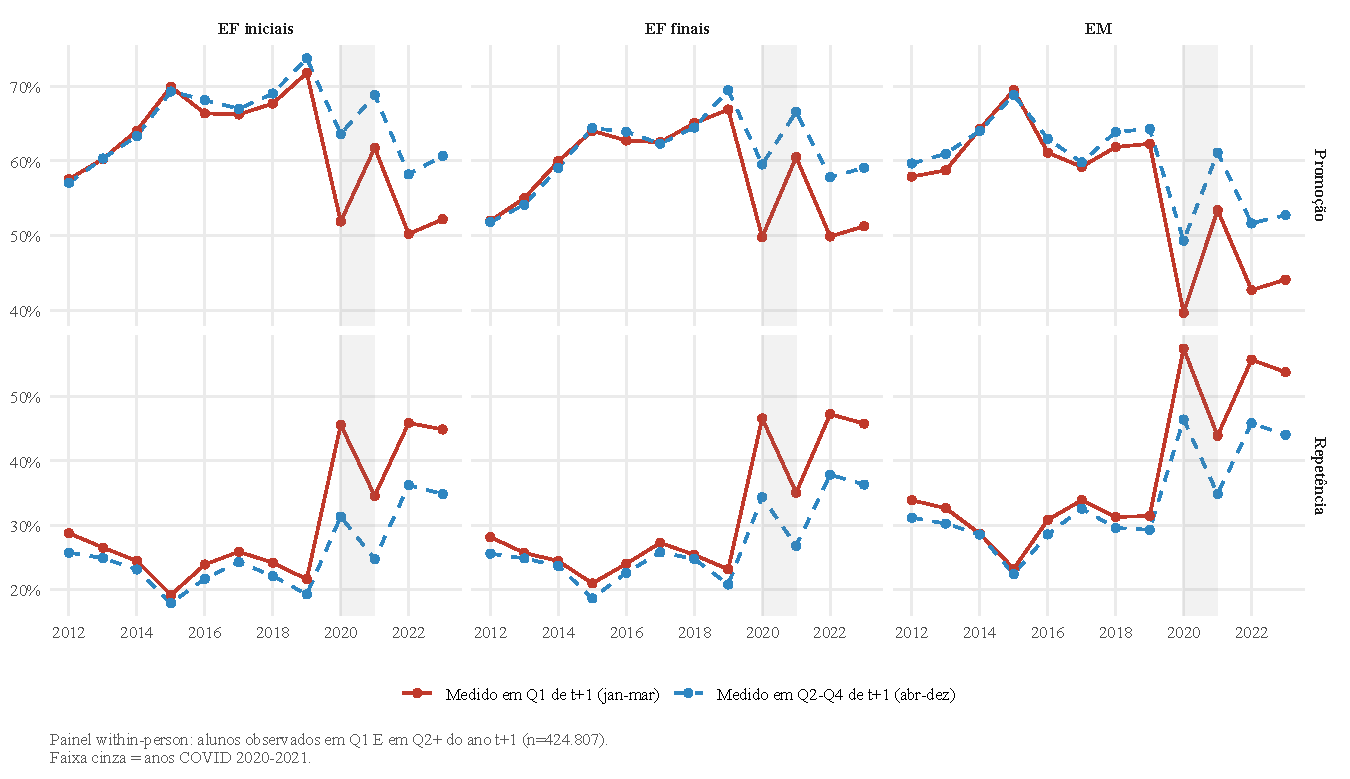
\includegraphics[width=0.95\textwidth]{../DataWork/5_Figures/output/F6_efeito_ferias_within.pdf}
\caption{Efeito do timing da observação de $t+1$ sobre promoção e
repetência (painel \emph{within-person}), por macroetapa.}
\label{fig:efeito_ferias}
\figurenote{Subamostra de alunos com observação em $Q_1$ e em algum
$Q \geq 2$ de $t+1$. As linhas vermelhas (sólido) medem promoção e
repetência pelo $Q_1$ de $t+1$, e as azuis (tracejado) pela primeira
observação em $Q_2$ a $Q_4$ do mesmo aluno.}
\end{figure}

A escolha da janela do indicador intra-ano foi testada em duas
variantes, a saber, primeira observação no ano $t$ contra última
observação no ano $t$, e visita $V_1$ contra visita $V_5$ por
indivíduo, e ambas produzem resultados estáveis. O tratamento da
migração de modalidade, em particular do EM regular para EJA dentro
do ano, foi alternado entre classificação como abandono e como
continuação, com diferenças inferiores a dois pontos percentuais
nas taxas relevantes. A idade-padrão para defasagem foi alternada
entre entrada aos seis anos e entrada aos sete anos no primeiro ano
do EF, sem alteração qualitativa dos resultados. As estimativas
principais da Tabela~\ref{tab:t1_brasil} são, em suma, estáveis a
essas variações, com diferenças menores que dois pontos
percentuais.

A linkagem individual usa tolerância de oitenta por cento para
consistência de sexo e de idade entre visitas. Como sensibilidade,
testamos duas variantes. Na variante \emph{strict}, exigimos cem
por cento de consistência, o que é mais conservador; na variante
\emph{loose}, aceitamos sessenta por cento de consistência,
recuperando mais indivíduos. A reponderação dos indicadores
principais sob essas variantes não move nenhum indicador além de
1,5 pontos percentuais, o que confirma a estabilidade do algoritmo
central. Para aproximadamente vinte por cento das transições
inter-ano, dispomos da Visita 5 da PNADC anual com a variável
\texttt{V5002A}, que indica recebimento de Bolsa Família. Nessa
subamostra, comparamos o perfil de fluxo dos indivíduos com BFA
observado contra os com perfil de renda compatível, mas sem BFA
observado. Os detalhes desta comparação serão preenchidos quando o
módulo B4 da estimação estiver completo.

A identidade contábil Promoção mais Repetência mais Evasão mais
Migração EJA igual a um deve ser aproximadamente satisfeita por
construção. Sob a metodologia v5, com a correção \texttt{V3014}
incorporada, a soma fica em torno de 98\% no EF iniciais e finais
e 97\% no EM. O resíduo de aproximadamente 2 a 3\% é atribuível a
transições para ensino superior, modalidades não classificadas e
casos limítrofes de matrícula em redes não cobertas pelo
\texttt{V3002A}. A PNADC mudou a codificação da
variável \texttt{V3003} em 2016, substituindo-a por \texttt{V3003A}
com códigos diferentes. A harmonização descrita no
Apêndice~\ref{app:variaveis} reconcilia os dois períodos. Para
validar, comparamos os indicadores das transições 2013/2014 e
2014/2015, pré-mudança, com 2016/2017 e 2017/2018, pós-mudança.
As séries são contínuas, sem descontinuidades visíveis na
Figura~\ref{fig:cohort_fluxo}, o que confirma que a harmonização
foi bem-sucedida.

% =========================================================================
% Secao 8 - Conclusoes e agenda
% =========================================================================

\section{Conclusões e agenda}
\label{sec:conclusao}

Esta nota propõe a construção de uma família de indicadores de
fluxo escolar, a saber, abandono, evasão, promoção, repetência,
migração para EJA e entrada no sistema, a partir do painel
longitudinal de cinco trimestres da PNAD Contínua. A literatura prévia brasileira sobre
fluxo escolar, em particular o trabalho do grupo PROFLUXO
\citep{Fletcher1985_modelo, Ribeiro1991_pedagogia,
KleinRibeiro1991_censo, Klein2006_educacao}, abordou o problema com
instrumentos diferentes, baseados em um modelo de fluxo de estado
estacionário aplicado a um corte transversal da PNAD. Esta nota não
é uma continuação ou extensão desse trabalho. Não há sobreposição
de autores e o arcabouço técnico é completamente distinto. O ponto
de contato é apenas o objeto comum, qual seja, usar pesquisa
domiciliar para medir fluxo escolar, e a importância histórica que
o PROFLUXO tem nas estatísticas educacionais brasileiras, em
particular a evidência apresentada por \cite{Ribeiro1991_pedagogia}
sobre a pedagogia da repetência no Brasil.

A análise mostra que a PNADC oferece quatro vantagens estruturais
sobre as estatísticas oficiais do INEP. A primeira é a
tempestividade, pois a PNADC é divulgada trimestralmente, com
defasagem máxima de quatro a cinco meses. Os Indicadores de
Trajetória do INEP, em contraste, são divulgados em ritmo errático,
com a última transição publicada, referente a 2021--2022, datada de
julho de 2025, e sem calendário público para atualizações
posteriores. Em meados de 2026, a defasagem do indicador mais
recente do INEP é de quatro anos, ao passo que a PNADC oferece
estimativas com defasagem inferior a um trimestre. A segunda
vantagem é a desagregação socioeconômica, pois a PNADC tem
variáveis individuais de renda, raça, idade, sexo e, na Visita 5,
recebimento de Bolsa Família. Os indicadores publicados pelo INEP
agregam apenas por etapa, rede, UF e localização urbana ou rural,
e os gradientes por quintil de renda e por perfil de elegibilidade
ao BFA documentados na Seção~\ref{sec:heterogeneidade} são, à data
desta nota, inviáveis com os dados publicados oficialmente. A
terceira vantagem é a independência da fonte, pois pesquisa
domiciliar e registro administrativo são metodologicamente
distintos, de modo que a convergência (ou a discrepância
controlada) entre os dois fortalece a confiança na medida e a
divergência sinaliza áreas onde o registro administrativo pode
estar viesado. Por fim, a quarta vantagem é a captura de retorno,
uma vez que a PNADC acompanha o indivíduo no domicílio, vendo
migrações entre redes, modalidades e UFs. A decomposição da
Seção~\ref{sec:inep} quantifica diretamente o componente $R$ do
\emph{gap} entre INEP e PNADC, ou seja, a fração de alunos
classificados como evadidos pelo Censo que continuam estudando
segundo a pesquisa domiciliar.

A abordagem proposta tem três limitações principais que devem
moderar a interpretação. A primeira diz respeito ao atrito do
painel. O acompanhamento longitudinal funciona apenas para
indivíduos que permanecem no mesmo domicílio, e indivíduos que
migram, por motivos como adolescentes que saem do domicílio dos
pais, casamentos ou óbitos, saem do painel. A
Seção~\ref{ssec:atrito} mostra que o atrito é correlacionado com
idade e renda, precisamente as dimensões mais relevantes para fluxo
escolar. Embora a reponderação por \emph{inverse propensity},
detalhada no Apêndice~\ref{app:variaveis}, corrija parte do viés,
esta é uma limitação inerente à pesquisa domiciliar. A segunda
limitação refere-se ao tamanho amostral em células finas. Para
subgrupos pequenos, como indígenas no EM por UF, a precisão das
estimativas é baixa, e recomendamos sempre reportar IC 95\% e
evitar agregações com $n < 100$. A terceira limitação diz respeito
ao conceito de frequência escolar. A variável \texttt{V3002} da
PNADC captura a situação na semana de referência, e em períodos de
férias ou paradas (o $Q_1$ do calendário civil é o início do ano
letivo brasileiro, e $Q_3$ e $Q_4$ abrigam férias escolares
parciais), a interpretação requer cuidado. Discutimos
especificamente esse ponto na Seção~\ref{ssec:efeito_ferias}.

A descontinuidade dos Indicadores de Trajetória do INEP cria um
vácuo informacional que esta nota busca preencher \emph{ad hoc}.
Em vista da relevância política e analítica das medidas de fluxo,
especialmente no contexto de políticas focalizadas como o
Pé-de-Meia \citep{Brasil2024_PeDeMeia}, o Bolsa Família e o
Auxílio Brasil, propomos uma sistematização institucional, isto é,
um Boletim Trimestral de Fluxo Escolar produzido com base na
PNADC, com periodicidade alinhada à divulgação dos microdados pelo
IBGE. O boletim seria, conceitualmente, o complemento contemporâneo
do PROFLUXO original, ou seja, usar pesquisa domiciliar para gerar
medidas longitudinais que o registro administrativo não consegue
manter. A diferença, agora, é que a observação substituiria o
modelo, e a frequência seria trimestral em vez de anual ou
plurianual.

A agenda subsequente inclui quatro frentes. A primeira é
aprofundar a comparação INEP \emph{versus} PNADC por UF e
macrorregião, em vez de apenas Brasil agregado. A segunda é
explorar o suplemento da quinta visita anual da PNADC, em
particular a variável \texttt{V5002A} de recebimento de Bolsa
Família, para análises com Bolsa Família observado em vez de
elegibilidade por renda, e variáveis adicionais sobre arranjo
familiar, gravidez e maternidade adolescente que ajudariam a
refinar a heterogeneidade da evasão. A terceira é estimar
efeitos do Pé-de-Meia sobre os indicadores de fluxo usando uma
estratégia de comparação antes e depois com controles em
coortes não-elegíveis, exercício que pertence a um próximo
trabalho. A quarta é replicar a abordagem para outros desfechos
educacionais, como frequência por modalidade EJA e transição
para o ensino superior. Em todos esses casos, a contribuição
metodológica desta nota, qual seja, usar o painel longitudinal
da PNADC como termômetro independente do fluxo escolar, é a
infraestrutura comum.


% ========================================================================
% Apendices
% ========================================================================
\appendix
% =========================================================================
% Apendice A - Tabelas detalhadas
% =========================================================================

\section{Tabelas detalhadas}
\label{app:uf}

Este apêndice apresenta tabelas detalhadas dos cinco indicadores de
fluxo escolar desagregados em dimensões adicionais àquelas
reportadas no corpo do texto. A
Tabela~\ref{tab:distorcao} reporta as taxas condicionais à
defasagem idade-série, comparando alunos em dia com alunos com
defasagem de pelo menos dois anos, para cada macroetapa. Os
números são médias 2018--2023, excluindo os anos COVID
(2020--2021). A tabela complementa a discussão da
Seção~\ref{sec:heterogeneidade} sobre o papel central da
defasagem idade-série como preditor de evasão.

% Auto-gerado por C16_distorcao_conditional.py
\begin{table}[htbp]
\centering
\caption{Taxas de fluxo condicionais \`a defasagem idade-s\'erie no in\'icio do painel, Brasil, m\'edia 2018--2023 (ex-COVID).}
\label{tab:distorcao}
\begin{threeparttable}
\small
\begin{tabular}{lrrrrrr}
\toprule
& \multicolumn{4}{c}{Taxas (\%)} & & \\
\cmidrule(lr){2-5}
Subgrupo & Promo\c{c}\~ao & Repet\^encia & Evas\~ao & Migra\c{c}\~ao EJA & Soma & N \\
\midrule
\multicolumn{7}{l}{\textit{EF iniciais}} \\
\midrule
Em dia & 79.5 & 18.7 & 0.1 & 0.0 & 98.3 & 38.619 \\
Defasagem $\geq 2$ anos & 73.0 & 20.3 & 3.3 & 1.3 & 97.9 & 3.653 \\
\\[0.3em]
\multicolumn{7}{l}{\textit{EF finais}} \\
\midrule
Em dia & 77.6 & 20.1 & 0.4 & 0.2 & 98.3 & 29.346 \\
Defasagem $\geq 2$ anos & 63.2 & 22.0 & 7.3 & 4.6 & 97.1 & 6.028 \\
\\[0.3em]
\multicolumn{7}{l}{\textit{EM}} \\
\midrule
Em dia & 51.2 & 19.5 & 19.6 & 0.3 & 90.6 & 19.097 \\
Defasagem $\geq 2$ anos & 34.0 & 18.6 & 37.1 & 4.9 & 94.6 & 4.282 \\
\bottomrule
\end{tabular}
\begin{tablenotes}\footnotesize
\item \textit{Fonte:} Painel longitudinal da PNADC.
\item \textit{Notas:} Defasagem idade-s\'erie computada como diferen\c{c}a entre idade observada e idade-padr\~ao (entrada aos 6 anos no 1\textsuperscript{o} EF). Defasagem $\geq 2$ anos: idade $\geq$ idade-padr\~ao $+\,2$.
\end{tablenotes}
\end{threeparttable}
\end{table}


Tabelas adicionais com os cinco indicadores desagregados por
unidade da federação, com intervalos de confiança \emph{bootstrap}
de 95\% (\emph{cluster} em UPA) serão preenchidas após a
finalização do processamento dos arquivos CSV correspondentes em
\texttt{DataWork/3\_Indicators/output/A1\_*}. Como o tamanho
amostral varia substancialmente entre UFs, células com $N < 30$
serão suprimidas e sinalizadas.

% =========================================================================
% Apendice B - Construcao das variaveis e codigos
% =========================================================================

\section{Construção das variáveis e códigos}
\label{app:variaveis}

Conforme discutido na Seção~\ref{sec:dados_metodo}, algumas variáveis
educacionais da PNADC mudaram de nome e de codificação ao longo do
período 2012--2024. A Tabela~\ref{tab:harmonizacao} na seção principal
lista os nomes das variáveis nas duas versões. A
Tabela~\ref{tab:codigos_v3003} a seguir detalha os mapeamentos de
valores entre as duas codificações para as duas variáveis mais
críticas, \texttt{V3003} pré-2016 e \texttt{V3003A} a partir de 2016.

\begin{table}[htbp]
\centering
\caption{Mapeamento de códigos: \texttt{V3003} (2012--2015) $\to$ \texttt{V3003A} (2016+).}
\label{tab:codigos_v3003}
\small
\begin{tabular}{cclc}
\toprule
\texttt{V3003} & \texttt{V3003A} & Curso/etapa frequentado & Macroetapa (esta nota) \\
\midrule
1 & 1 & Creche                                          & ---             \\
2 & 2 & Pré-escola                                      & ---             \\
3 & 4 & Regular Fundamental                             & EF iniciais / finais \\
4 & 5 & EJA Fundamental                                 & EJA EF          \\
5 & 6 & Regular Médio                                   & EM              \\
6 & 7 & EJA Médio                                       & EJA EM          \\
7 & 8 & Educação Profissional (médio)                   & EM (técnico)    \\
8 & 10 & Superior - graduação                           & ---             \\
9 & 11 & Especialização (nível superior)                & ---             \\
10 & 12 & Mestrado                                      & ---             \\
11 & 13 & Doutorado                                     & ---             \\
--- & 3  & Alfabetização de jovens e adultos            & EJA EF          \\
--- & 9  & Educação Profissional (qualif.\ profissional) & ---             \\
\bottomrule
\end{tabular}
\end{table}

A discrepância crítica é o deslocamento de uma unidade para os códigos
maiores ou iguais a três a partir de 2016, decorrente da inserção de
novas categorias, especificamente da ``Alfabetização de jovens e
adultos'', código 3 na nova versão. Sem a harmonização, alunos
classificados como ``Regular Fundamental'' em 2012--2015 (código 3
em \texttt{V3003}) seriam erroneamente classificados como
``Alfabetização'' (código 3 em \texttt{V3003A}) caso as variáveis
fossem empilhadas sem ajuste, erro que afeta cerca de noventa e cinco
por cento das observações pré-2016 em idade escolar EF. A variável de
série, \texttt{V3006}, é estável em todo o período 2012--2024.
Codifica o ano que o indivíduo cursa, no formato $XYY$, em que $X$ é
o nível (1 para Fundamental, 2 para Médio, 3 para Superior e 4 para
outros) e $YY$ é o ano (01 a 09 para EF e 01 a 04 para EM). Por
exemplo, \texttt{V3006=108} identifica o oitavo ano do EF. A
variável \texttt{V3006A}, introduzida em 2016, acrescenta a
desagregação ``EF anos iniciais'' (1 a 5) e ``EF anos finais'' (6 a
9), redundante com \texttt{V3006} mas conveniente para filtros.

O identificador domiciliar estável é construído como a concatenação
$\texttt{hh\_id} = \texttt{UF} \,\|\, \texttt{UPA} \,\|\, \texttt{V1008} \,\|\, \texttt{V1014}$,
e o identificador individual pré-validação é
$\texttt{pid} = \texttt{hh\_id} \,\|\, \texttt{V2003}$. Após a
validação de consistência por sexo e idade, elos com inconsistência
em vinte por cento ou mais das visitas são marcados como elo
quebrado e descartados do painel. Para corrigir possível viés de
atrito, estimamos a propensão de retenção como
\[
\Pr(R_i = 1 \mid X_i) = \Phi(X_i' \beta),
\]
em que $R_i \in \{0,1\}$ indica retenção do indivíduo $i$ no painel
entre as duas visitas usadas no indicador, e $X_i$ inclui idade,
idade ao quadrado, sexo, raça, renda per capita, logaritmo da renda
per capita, rede da escola, UF (efeito fixo) e trimestre da primeira
observação (efeito fixo). O peso corrigido por \emph{inverse
propensity}, denominado P3, é
\[
w_i^{P3} = w_i^{P1} \cdot \frac{1}{\hat\Pr(R_i=1 \mid X_i)}.
\]

Toda a análise é reprodutível usando o código disponível em
\href{https://github.com/vitpereira/Nota_PNAD}{github.com/vitpereira/Nota\_PNAD}
(a ser publicado na submissão). O \emph{stack} computacional é
composto por Python para o \emph{parse} dos microdados, Stata 19
para a construção do painel e o cálculo dos indicadores e R com
\emph{ggplot2} para as figuras. Sementes aleatórias estão fixadas
para garantir a reprodutibilidade dos testes Monte Carlo. Para
facilitar a replicação e a aplicação desta metodologia em outros
contextos, disponibilizamos um pacote R público em
\href{https://github.com/vitpereira/fluxoescolar}{github.com/vitpereira/fluxoescolar}.
O pacote oferece oito funções exportadas, a saber,
\texttt{baixar\_pnadc()} para download direto do FTP do IBGE,
\texttt{parsear\_pnadc()} para \emph{parse} dos microdados
fixed-width, \texttt{harmonizar\_pnadc()} para consolidação dos
códigos pré e pós 2016, \texttt{construir\_painel()} para linkagem
individual via Ribas-Soares, \texttt{calcular\_indicadores()} para
cálculo dos cinco indicadores, \texttt{decompor\_inep()} para a
decomposição $R+U+S+C+M$, e duas funções de visualização. O pacote
inclui testes unitários, \emph{vignette} introdutória e fluxo de
CI via GitHub Actions, e pode ser instalado via\\
\texttt{remotes::install\_github("vitpereira/fluxoescolar")}.


% ========================================================================
% Referencias
% ========================================================================
\newpage
\singlespacing
\bibliographystyle{plainnat}
\bibliography{../Bibliography_base}

\end{document}
